\documentclass[]{beamer}
%\documentclass[handout]{beamer}
\usetheme{Boadilla} 
%\usecolortheme{seagull}
%\setbeamerfont*{frametitle}{size=\normalsize,series=\bfseries}
%\setbeamertemplate{blocks}[default]%[shadow=false]

\setbeamertemplate{footnote}{\tiny\makebox[1em][l]{\insertfootnotemark}\insertfootnotetext\par}



%\setbeamertemplate{footnote}{\hangpara{1em}{1}\makebox[1em][l]{\insertfootnotemark}\scriptsize\insertfootnotetext\par}

%\definecolor{icml_tutorial}{RGB}{181,74,16}

%\setbeamercolor{title}{bg=icml_tutorial,fg=white}

%\usetheme{Boadilla}
\usefonttheme{professionalfonts}
%%\usecolortheme{seagull}
\usefonttheme[onlymath]{serif}
%
\setbeamertemplate{blocks}[rounded][shadow=false]

\usepackage{array}
%\usepackage{algorithm}
%\usepackage{algorithmic}
%\usepackage[english]{babel}
\usepackage{booktabs} 
\usepackage{graphicx}
\usepackage{amssymb}
\usepackage{amsmath}
\usepackage{stmaryrd} 
\usepackage{dsfont}
\usepackage{color,colortbl} 
\usepackage{pgfplots}
%\usepackage{bibentry}
\usepackage{algorithm}
\usepackage[noend]{algpseudocode}
\usepackage{tikz}
\usetikzlibrary{mindmap,trees}
\usetikzlibrary{decorations.pathreplacing}
\usetikzlibrary{decorations.pathmorphing}
\usetikzlibrary{arrows}
\usetikzlibrary{positioning}
\usetikzlibrary{decorations.text}
\usetikzlibrary{decorations.markings}
\usetikzlibrary{decorations.shapes}
\usetikzlibrary{shapes,snakes}
\usetikzlibrary{calc,trees,positioning,arrows,chains,shapes.geometric,
  decorations.pathreplacing,decorations.pathmorphing,shapes,matrix,shapes.symbols}
\usetikzlibrary{shapes.misc}

\usepackage{multirow}
% \usepackage{beamerthemesplit} // Activate for custom appearance



 
\newcommand{\lsize}{m}
\newcommand{\osize}{n}
\newcommand{\qsize}{q}
\newcommand{\odsize}{d}
\newcommand{\qdsize}{r}
\newcommand{\ispace}{\mathcal{X}}
\newcommand{\taskspace}{\mathcal{T}}
\newcommand{\objspace}{\mathcal{D}}
\newcommand{\anyspace}{\mathcal{X}}
\newcommand{\hypspace}{\mathcal{H}}
\newcommand{\kernelf}{k}
\newcommand{\gkernelf}{g}
\newcommand{\kkernelf}{\Gamma}
\newcommand{\dkernelm}{\bm{K}}
\newcommand{\tkernelm}{\bm{G}}
\newcommand{\kkernelm}{\bm{\Gamma}}
\newcommand{\regparam}{\lambda}
\newcommand{\idmatrix}{\bm{I}}
\newcommand{\trace}{\textnormal{tr}}
%\newcommand{\transpose}{^\textnormal{T}}
\newcommand{\transpose}{^\intercal}
\newcommand{\bm}[1]{\mathbf{#1}}
\newcommand{\ve}{\textnormal{vec}}
\newcommand{\mat}{\textnormal{mat}}
\newcommand{\diagv}{\textnormal{diag}_v}
\newcommand{\diagm}{\textnormal{diag}_m}
\newcommand{\LOO}{\text{LOO}}
\newcommand{\predfun}{f}
\newcommand{\filterfun}{\varphi}
\newcommand{\objset}{D}
\newcommand{\taskset}{T}
\newcommand{\labelvec}{\bm{y}}
\newcommand{\Algo}[1]{{#1}}


\setbeamertemplate{footline}[frame number]
\beamertemplatenavigationsymbolsempty 
%\logo{
\includegraphics[height=1.2cm]{Figures/Kermit}}



\renewcommand{\Pr}{P}
\newcommand{\cumPr}{\mathbf{P}}
\renewcommand{\vec}[1]{\boldsymbol{#1}}
\newcommand{\brY}{\vec{Y}}
\newcommand{\given}{\, | \,}
\newcommand{\cumprob}{P}
\newcommand{\cumprobx}{P_{\vec{x}}}
\newcommand{\probx}{p_{\vec{x}}}
\newcommand{\probxi}[1]{p_{\vec{x}}^{(#1)}}
\newcommand{\invmarg}[1]{P_{\vec{x},#1}^{-1}}
\newcommand{\cop}{C}
\newcommand{\dcop}{c}
\newcommand{\copx}{C_{\vec{x}}}
\newcommand{\dcopx}{c_{\vec{x}}}
\newcommand{\mx}[1]{\mathbf{\mathrm{#1}}}
\newcommand{\maxprobxi}[1]{p_{\vec{x},max}^{(#1)}}
\newcommand{\minprobxi}[1]{p_{\vec{x},min}^{(#1)}}
\DeclareMathOperator*{\argmax}{\arg \max}
\DeclareMathOperator*{\argmin}{\arg \min}

\newcommand{\Fb}{F}
\newcommand{\loss}{L}
\newcommand{\ells}{\tilde{\ell}}
\newcommand{\regret}{\textnormal{Reg}}
\newcommand{\lossrank}{L_{\textnormal{\scriptsize{rnk}}}}
\newcommand{\ellrank}{\ell_{\textnormal{\scriptsize{rnk}}}}
\newcommand{\regretrank}{{\textnormal{Reg}}_{\textnormal{\scriptsize{rnk}}}}
%\newcommand{\lossranktilde}{L_{\widetilde{rnk}}}
%\newcommand{\regretranktilde}{{\textnormal{Reg}}_{\widetilde{rnk}}}
\newcommand{\lossranktilde}{\lossrank}
\newcommand{\regretranktilde}{\regretrank}
\newcommand{\lossexp}{L_{\textnormal{\scriptsize{exp}}}}
\newcommand{\ellexp}{\ells_{\textnormal{\scriptsize{exp}}}}
\newcommand{\regretexp}{{\textnormal{Reg}}_{\textnormal{\scriptsize{exp}}}}
\newcommand{\losslog}{L_{\textnormal{\scriptsize{log}}}}
\newcommand{\elllog}{\ells_{\textnormal{\scriptsize{log}}}}
\newcommand{\regretlog}{{\textnormal{Reg}}_{\textnormal{\scriptsize{log}}}}
\newcommand{\lossrankbar}{L_{\textnormal{\scriptsize{br}}}}
\newcommand{\ellrankbar}{\ell_{\textnormal{\scriptsize{br}}}}
\newcommand{\regretrankbar}{{\textnormal{Reg}}_{\textnormal{\scriptsize{br}}}}

\newcommand{\sgn}[1]{\textrm{sgn}\left(#1\right)}
%\newcommand{\bm}{\mathds{1}}
\newcommand{\ZO}{0/1 }
\newcommand{\bx}{\boldsymbol{x}}
\newcommand{\by}{\boldsymbol{y}}
\newcommand{\bh}{\boldsymbol{h}}
\newcommand{\bY}{\boldsymbol{Y}}
\newcommand{\bX}{\boldsymbol{X}}
\newcommand{\bz}{\boldsymbol{z}}
%\newcommand{\bm}{\mathds{1}}
\newcommand{\assert}[1]{\llbracket #1 \rrbracket}
%\newcommand{\assert}[1]{\bm [ #1 ] } %[\llbracket #1 \rrbracket}
\newcommand{\colorcell}{\multicolumn{1}{>{\columncolor{DarkGreen}}l}{}}
\newcommand{\graytextcell}[1]{\begin{color}{gray}#1\end{color}}
\newcommand{\calX}{\mathcal{X}}
\newcommand{\calY}{\mathcal{Y}}
\newcommand{\calH}{\mathcal{H}}
\newcommand{\calL}{\mathcal{L}}
\newcommand{\calO}{\mathcal{O}} 
\newcommand{\calC}{\mathcal{C}} 

%\newcommand{\loss}{L}
%\newcommand{\regret}{\textnormal{Reg}}
\newcommand{\lossell}{L_{\ell}}
\newcommand{\regretell}{\textnormal{Reg}_{\ell}}
%\newcommand{\lossrank}{L_{\textnormal{\scriptsize{rank}}}}
%\newcommand{\regretrank}{{\textnormal{Reg}}_{\textnormal{\scriptsize{rank}}}}
%\newcommand{\sgn}[1]{\textrm{sgn}\left(#1\right)}
%\newcommand{\bm}{\mathds{1}}

\definecolor{putblue}{RGB}{0,0,124}
\definecolor{putred}{RGB}{204,33,69}
\renewcommand{\alert}[1]{\textbf{\color{putblue} #1}}
\renewcommand{\emph}[1]{\textbf{\color{putblue}#1}}
%\renewcommand{\emph}[1]{\textbf{\color{icml_tutorial}#1}}


\setbeamercolor{title}{bg=white,fg=putblue}
\setbeamercolor{subtitle}{bg=white,fg=putblue}

%\newcommand {\autographics}[1] {
  %\begin{center}
    %\includegraphics[width=\textwidth,height=0.85\textheight,keepaspectratio]{#1}
  %\end{center}
%}
%\newcommand {\autographicswithsize}[2] {
  %\begin{center}
    %\includegraphics[width=\textwidth,height=#2\textheight,keepaspectratio]{#1} 
  %\end{center}
%}

%\newcommand {\autographicswithsizew}[2] {
  %\begin{center}
  %\vskip-20pt
    %\includegraphics[width=\textwidth,width=#2\textheight,keepaspectratio]{#1}
  %\vskip5pt
  %\end{center}
%}

%\def\newblock{\hskip .11em } %plus .33em minus .07em}


\title[]{Multi-Target Prediction:\\ 
A Unifying View on Problems and Methods}
\author[Willem Waegeman]{Willem Waegeman and Dimitrios Iliadis} 
%\author[Eyke]{Eyke H\"ullermeier}
%\date[NIPS 2015]{NIPS: extreme classification workshop\\December 12, 2015}
\institute[VFU] % (optional)
{
  \inst{}
Department of Data Analysis and Mathematical Modelling, Ghent University, Belgium
}

%\date{Winter School on Machine Learning, Gran Canaria, 2020 }

\begin{document}

\frame{\titlepage}


\section{Introduction}

%\begin{frame}[plain]
        %\begin{tikzpicture}[remember picture,overlay]
            %\node[at=(current page.center)] {
                %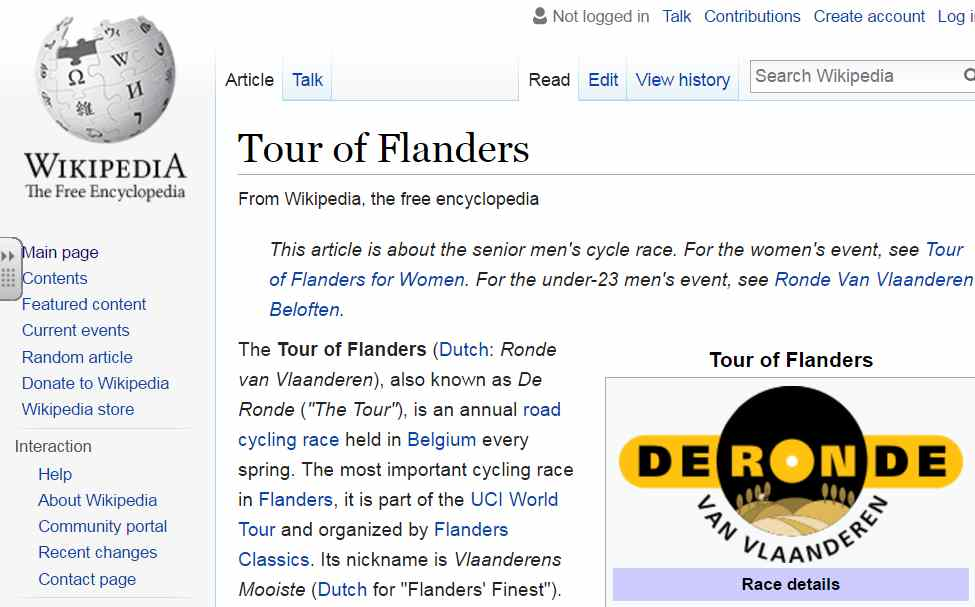
\includegraphics[scale=0.35]{pics/flanders}
            %};
        %\end{tikzpicture}
     %\end{frame}
		
		\begin{frame}[plain]
        \begin{tikzpicture}[remember picture,overlay]
            \node[at=(current page.center)] {
                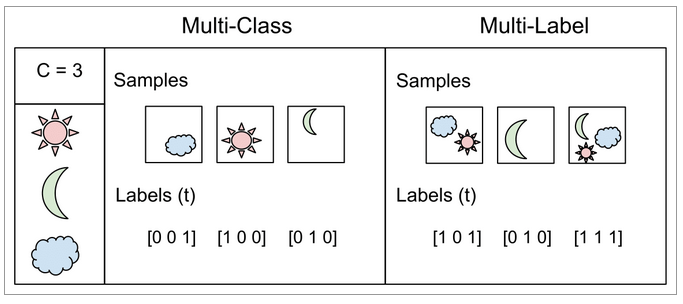
\includegraphics[scale=0.5]{pics/multi-classlabel}
            };
        \end{tikzpicture}
     \end{frame}

%\section{Introduction}


\begin{frame}{Multi-label classification: \\
the example of document categorization}
% voorbeeldje met boeken
\includegraphics[scale=0.17]{pics/kompany}
\end{frame}

\begin{frame}{Multi-label classification: \\
the example of document categorization}
% voorbeeldje met boeken
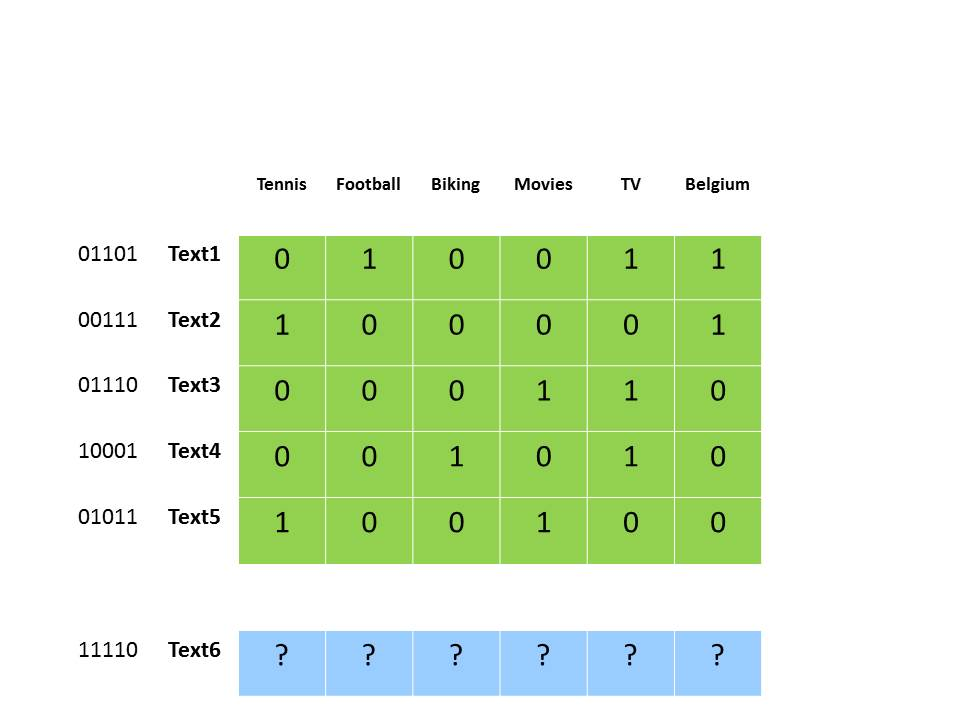
\includegraphics[width=0.9\textwidth,trim = 0 0 100 100,clip]{Figures/pictures/Slide2}
\end{frame}

\begin{frame}[plain]
        \begin{tikzpicture}[remember picture,overlay]
            \node[at=(current page.center)] {
                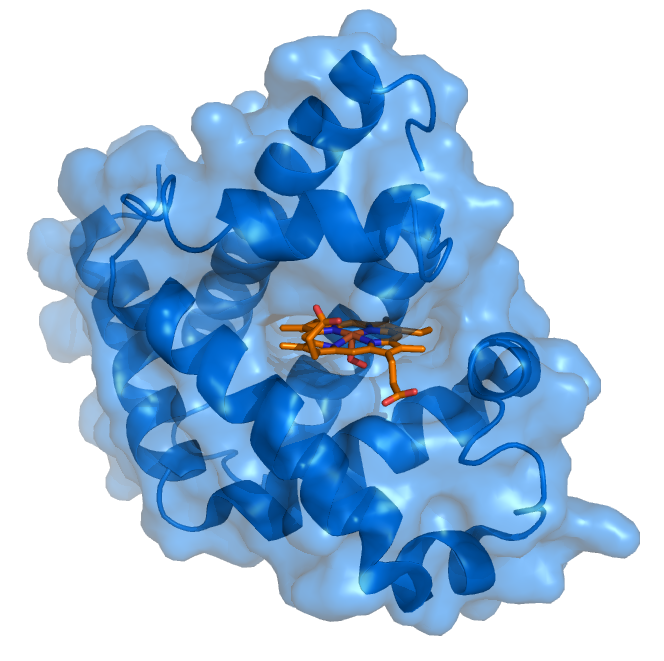
\includegraphics[width=0.7\textwidth]{pics/proteinl}
            };
        \end{tikzpicture}
     \end{frame}

\begin{frame}{Multivariate regression: \\
the example of protein-ligand interaction prediction}
% voorbeeldje met boeken
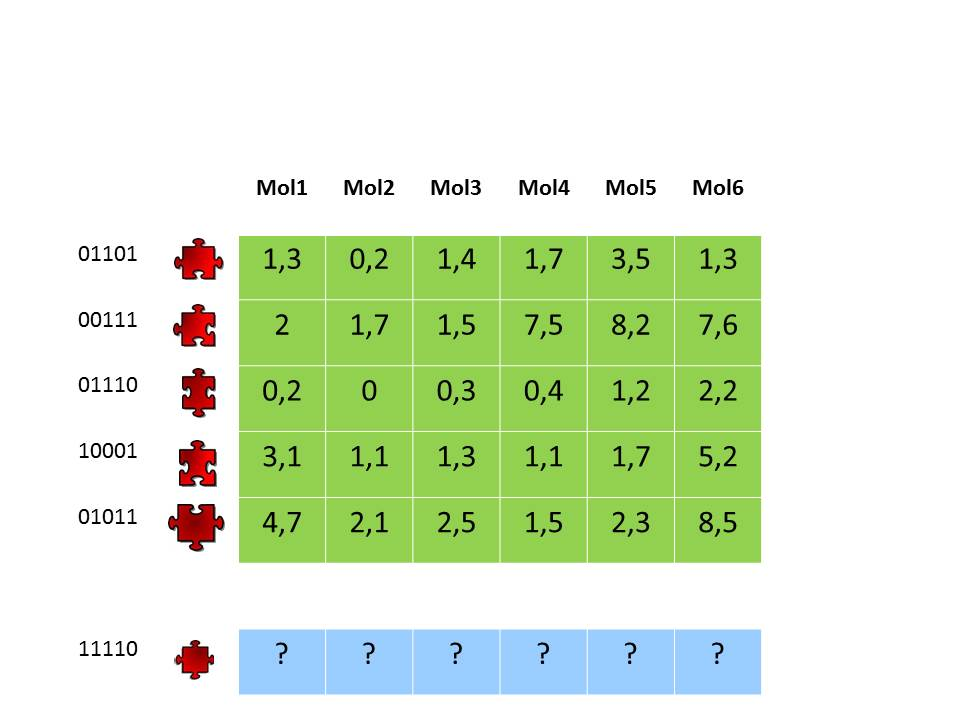
\includegraphics[width=0.9\textwidth,trim = 0 0 100 100,clip]{Figures/pictures/Slide1}
\end{frame}

\begin{frame}[plain]
        \begin{tikzpicture}[remember picture,overlay]
            \node[at=(current page.center)] {
                
\includegraphics[width=\textwidth]{Figures/school_shopping}
            };
        \end{tikzpicture}
     \end{frame}

\begin{frame}{Multi-task learning: \\
the example of predicting student marks}
% voorbeeldje met boeken
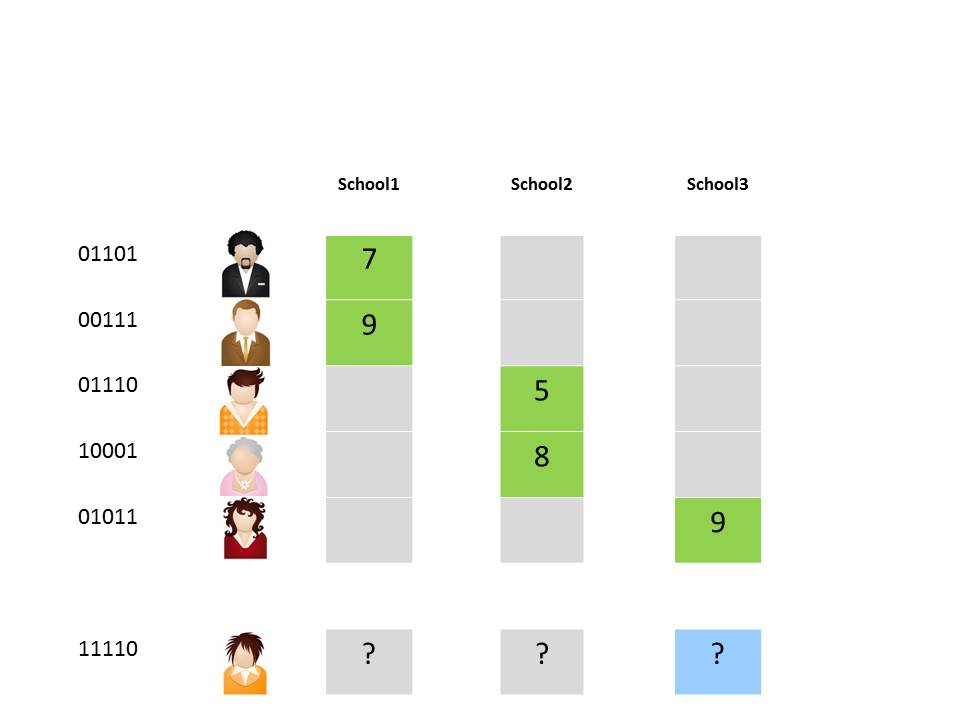
\includegraphics[width=0.9\textwidth,trim = 0 0 100 100,clip]{Figures/pictures/Slide3}
\end{frame}



%\begin{frame}{Other cool applications: ecology}
   %\center 
   %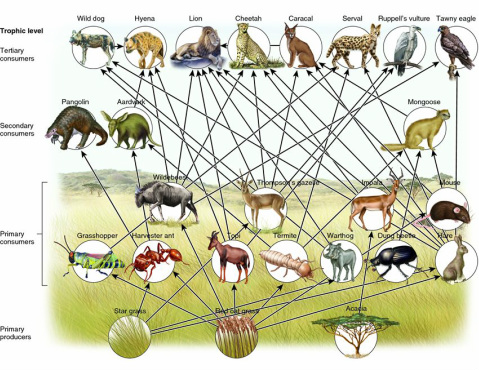
\includegraphics[width=10cm]{Figures/foodweb.jpg}
   %\vfill
   %%Predicting links between \alert{people}
 %% social network prediction, protein ligand prediction, food pairing, image analysis: voorbeeld?
%\end{frame}

%\begin{frame}{Other cool applications: food pairing}
   %\center 
   %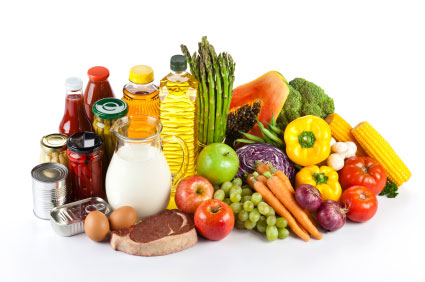
\includegraphics[width=\textwidth]{Figures/ingredients}
   %\vfill
 %% social network prediction, protein ligand prediction, food pairing, image analysis: voorbeeld?
%\end{frame}

%
%\begin{frame}{The two-step ridge regression}
%Prediction function:
%
%$$
%f(d, t) = \boldsymbol{\phi}(d)^\intercal\mathbf{W}  \boldsymbol{\psi}  (t) 
%$$
%
%Parameters can be found by solving:
%$$
%\boldsymbol{\Phi}^\intercal\mathbf{Y}\boldsymbol{\Psi} = (\boldsymbol{\Phi}^\intercal\boldsymbol{\Phi}+\lambda_d\mathbf{I})\mathbf{W}(\boldsymbol{\Psi}^\intercal\boldsymbol{\Psi}+\lambda_t\mathbf{I})
%$$
%\pause
%Two hyperparameters: $\lambda_d$ and $\lambda_t$!
%\end{frame}

\begin{frame}{There are a lot of multi-target prediction problems around...}

\begin{center}
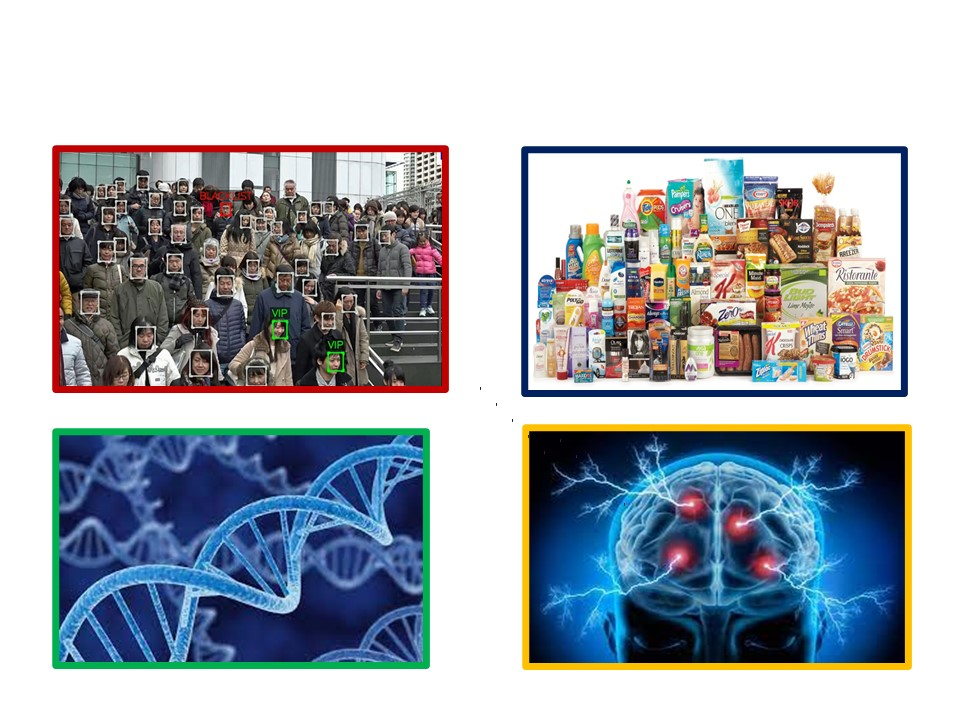
\includegraphics[width=\textwidth,trim = 0 0 0 70,clip]{Figures/pictures/Slide25}
\end{center}

\end{frame} 

\begin{frame}{Matrix completion: a recommender system}

\begin{center}
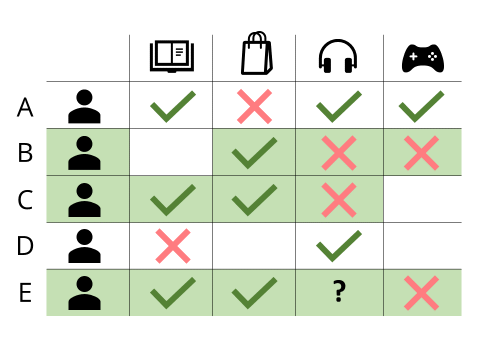
\includegraphics[scale=0.5]{Figures/collafilt}
\end{center}

\end{frame}

\begin{frame}{Matrix completion: a genomics example}

\begin{center}
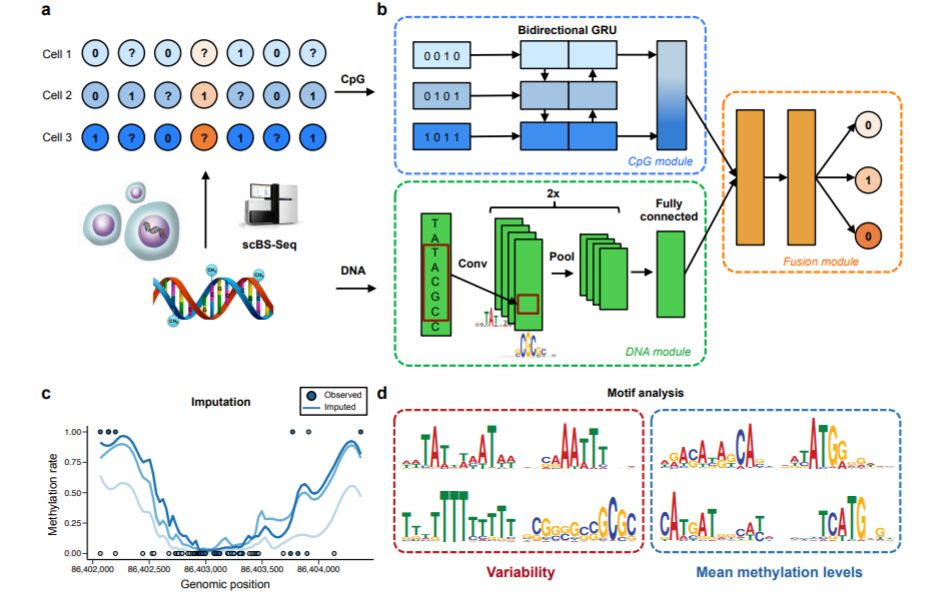
\includegraphics[scale=0.3]{Figures/deepcpg} \\
Angermueller et al.\ Accurate prediction of single-cell DNA methylation states
using deep learning, Genome Biology, 2017.

\end{center}

\end{frame}

\begin{frame}{Multi-task learning: detecting epileptic seizures}
% voorbeeldje met boeken
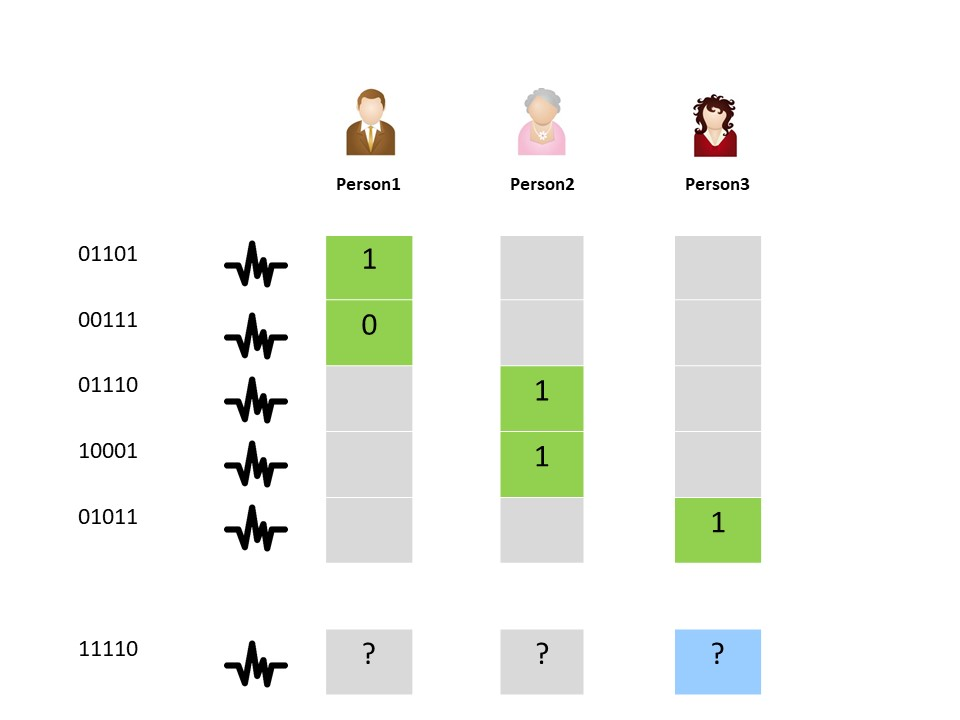
\includegraphics[width=0.9\textwidth,trim = 0 0 100 50,clip]{Figures/pictures/Slide24}
\end{frame}


\begin{frame}{Accompanying article}

\begin{center}
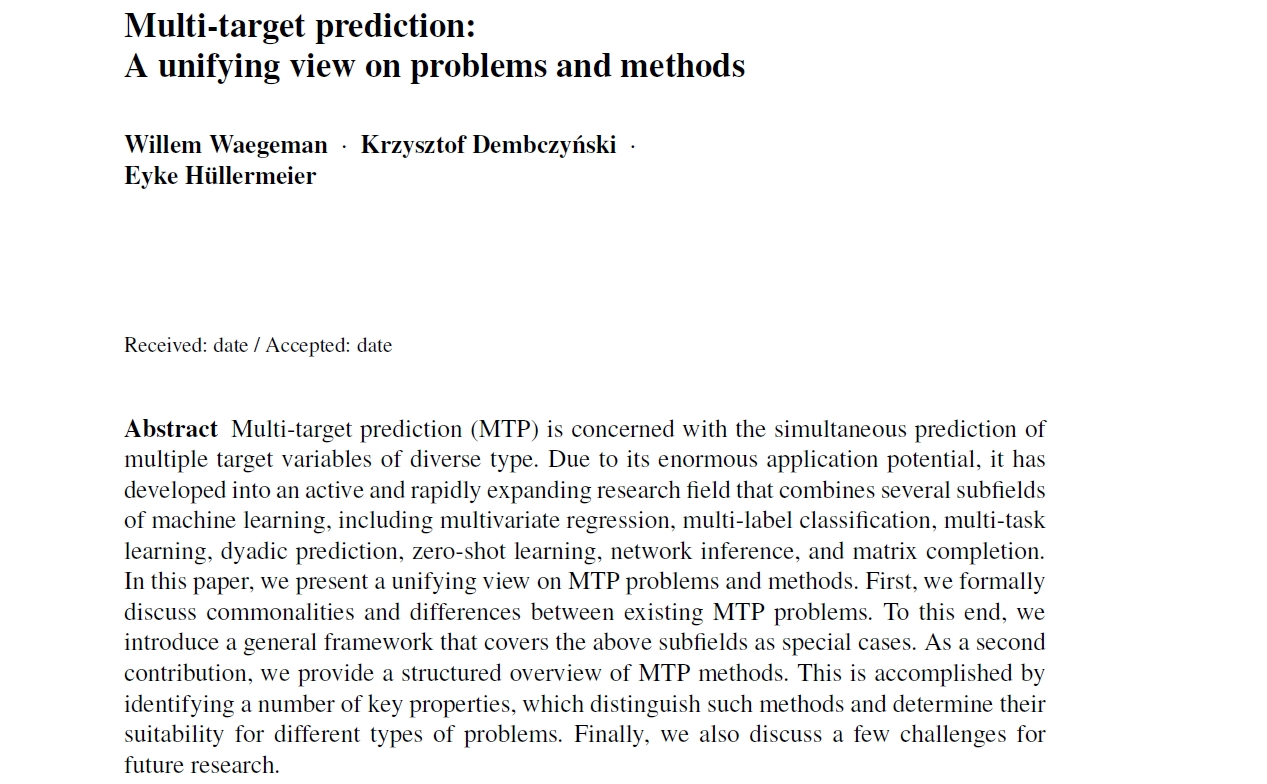
\includegraphics[width=\textwidth,trim = 0 0 0 0,clip]{Figures/dami}\\
Data Mining and Knowledge discovery, 2019. 
\end{center}

\end{frame}


%%% begin changes %%%


\section{A unifying view on MTP problems}


\begin{frame}{Overview of this talk}

\tableofcontents

\end{frame}




%\begin{frame}
%\frametitle{Multi-target prediction}
%\begin{itemize}
%\item \emph{Multi-Target Prediction:} For a feature vector $\bx$ predict accurately \\a vector of responses $\by$ using a function $\bh(\bx)$:
%$$
%\bx = (x_1,x_2,\ldots,x_p) \xrightarrow{~~\bh(\bx)~~} \by = (y_1, y_2, \ldots, y_m)
%$$
%\item \emph{Main challenges:} 
%\begin{itemize}
%\item Appropriate modeling of target dependencies between targets 
%$$
%y_1, y_2, \ldots, y_m
%$$
%\item A multitude of multivariate loss functions defined over the output vector 
%$$\ell(\by, \bh(\bx))$$
%%to measure the quality of prediction.
%\end{itemize}
%\item \emph{Main question:} %Can we improve over independent models trained for each target?
%\begin{itemize}
%\item Can we improve over independent models trained for each target? 
%\end{itemize}
%\item \emph{Two views:} %the individual target and joint target view.
%\begin{itemize}
%\item The individual-target view
%\item The joint-target view
%\end{itemize}
%\end{itemize}
%
%\end{frame}

\begin{frame}{General framework}
\begin{definition}
A multi-target prediction setting is characterized by instances $\vec{x} \in \mathcal{X}$ and targets $\vec{t} \in \mathcal{T}$ with the following properties: 
\begin{itemize} 
\item[1.] A training dataset consists of triplets $(\vec{x}_i,\vec{t}_j,y_{ij})$, where $y_{ij} \in \mathcal{Y}$.  
\item[2.] In total $n$ instances and $m$ targets are observed during training, with $n$ and $m$ finite numbers. 
\item[3.]As such, the scores $y_{ij}$ of the training data can be arranged in an $n \times m$ matrix $Y$.
\item[4.] The score set $\mathcal{Y}$ is one-dimensional. It consists of nominal, ordinal or real values.  
\item[5.] The goal consists of making predictions for any instance-target couple $(\vec{x},\vec{t}) \in \mathcal{X} \times \mathcal{T}$.   
\end{itemize}
\end{definition}
\end{frame}

\begin{frame}{Conventional MTP settings}
\begin{itemize}
\item Side information for targets is normally not available. 
\item \emph{Multi-label classification} (e.g., assigning appropriate category tags to documents).
\item \emph{Multivariate regression} (e.g., predicting whether a protein will bind to a set of experimentally developed small molecules).
\item \emph{Multi-task learning} (e.g., predicting student marks in the final exam for a typical high-school course).
\end{itemize}
\end{frame}





\begin{frame}{Conventional MTP settings}
\begin{definition}[Multi-label classification] 
A multi-label classification problem is a specific instantiation of the general framework, which exhibits the following additional properties: 
\begin{enumerate}
\item[P5.] The cardinality of $\mathcal{T}$ is $m$; this implies that all targets are observed during training. 
\item[P6.] No side information is available for targets. Again, without loss of generality, we can hence identify targets with natural numbers, such that the target space is $\mathcal{T} = \{1,...,m\}$. 
\item[P7.] The score matrix $Y$ has no missing values. 
\item[P8b.] The score set is $\mathcal{Y} = \{0,1\}$. 
\end{enumerate}
\end{definition}
\end{frame}

\begin{frame}{Multi-label classification}
% voorbeeldje met boeken
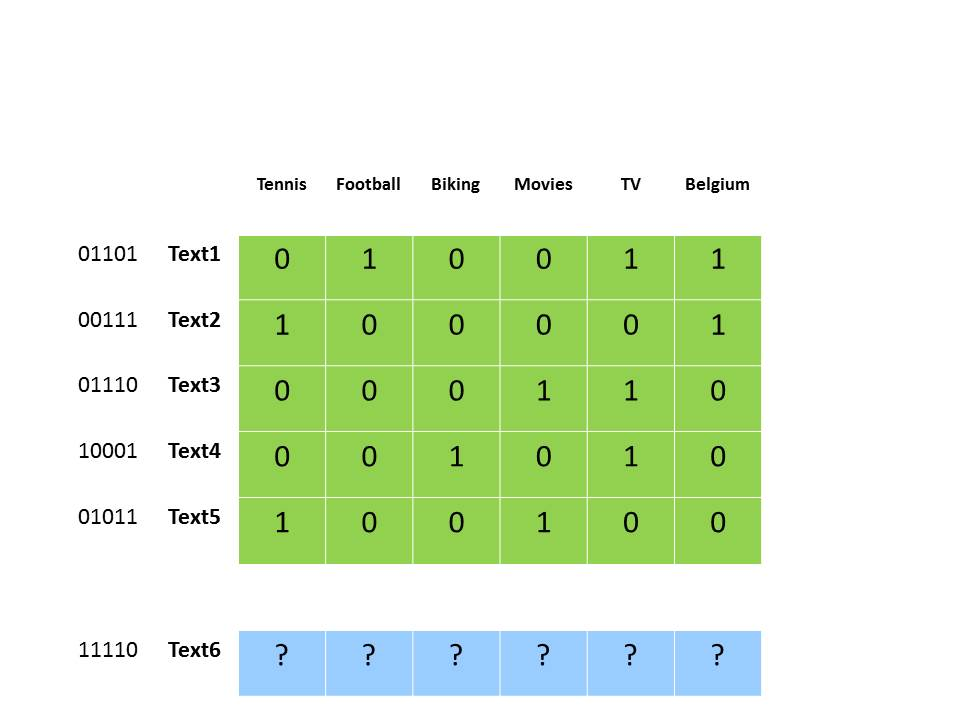
\includegraphics[width=0.9\textwidth,trim = 0 0 100 100,clip]{Figures/pictures/Slide2}
\end{frame}

\begin{frame}{Conventional MTP settings}
\begin{definition}[Multivariate regression] 
A multivariate regression problem is a specific instantiation of the general framework, which exhibits the following additional properties: 
\begin{enumerate}
\item[P5.] The cardinality of $\mathcal{T}$ is $m$. This implies that all targets are observed during training. 
\item[P6.] No side information is available for targets. Without loss of generality, we can hence assign the numbers $1$ to $m$ as identifiers to targets, such that the target space is $\mathcal{T} = \{1,...,m\}$. 
\item[P7.] The score matrix $Y$ has no missing values. 
\item[P8.] The score set is $\mathcal{Y} = \mathbb{R}$. 
\end{enumerate}
\end{definition}
\end{frame}

\begin{frame}{Multivariate regression}
% voorbeeldje met boeken
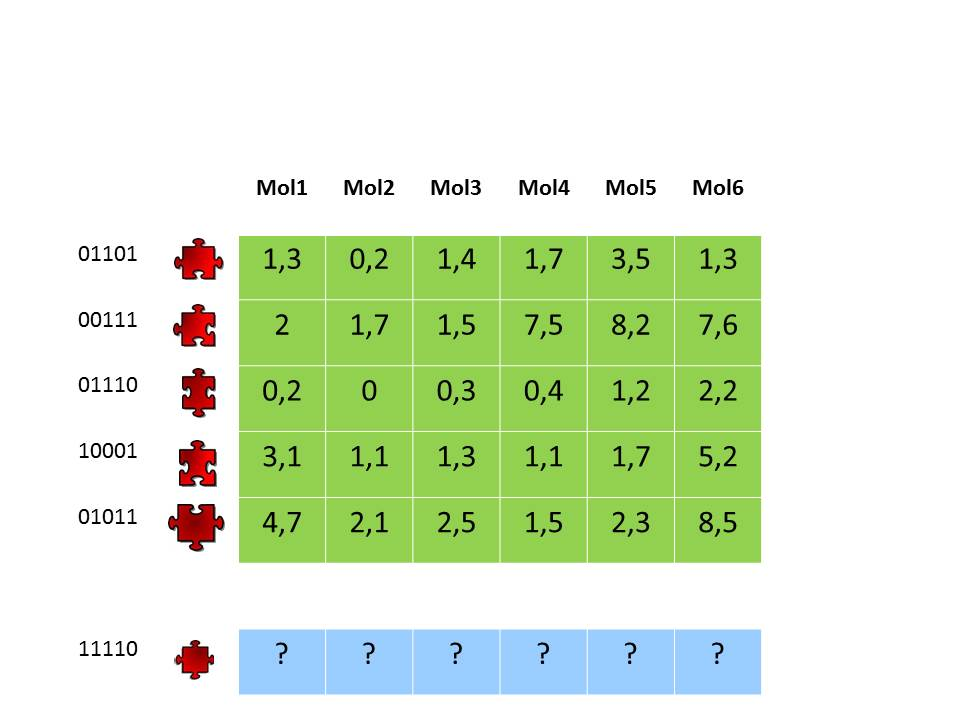
\includegraphics[width=0.9\textwidth,trim = 0 0 100 100,clip]{Figures/pictures/Slide1}
\end{frame}

\begin{frame}{Conventional MTP settings}
\begin{definition}[Multi-task learning] 
A multi-task learning problem is a specific instantiation of the general framework, which exhibits the following additional properties: 
\begin{enumerate}
\item[P5.] The cardinality of $\mathcal{T}$ is $m$; this implies that all targets are observed during training. 
\item[P6.] No side information is available for targets. Again, the target space can hence be taken as $\mathcal{T} = \{1,...,m\}$.   
\item[P8a.] The score set is homogenous across columns of $Y$, e.g., $\mathcal{Y} = \{0,1\}$ or $\mathcal{Y} = \mathbb{R}$.
\end{enumerate}
\end{definition}
\end{frame}


\begin{frame}{Multi-task learning}
% voorbeeldje met boeken
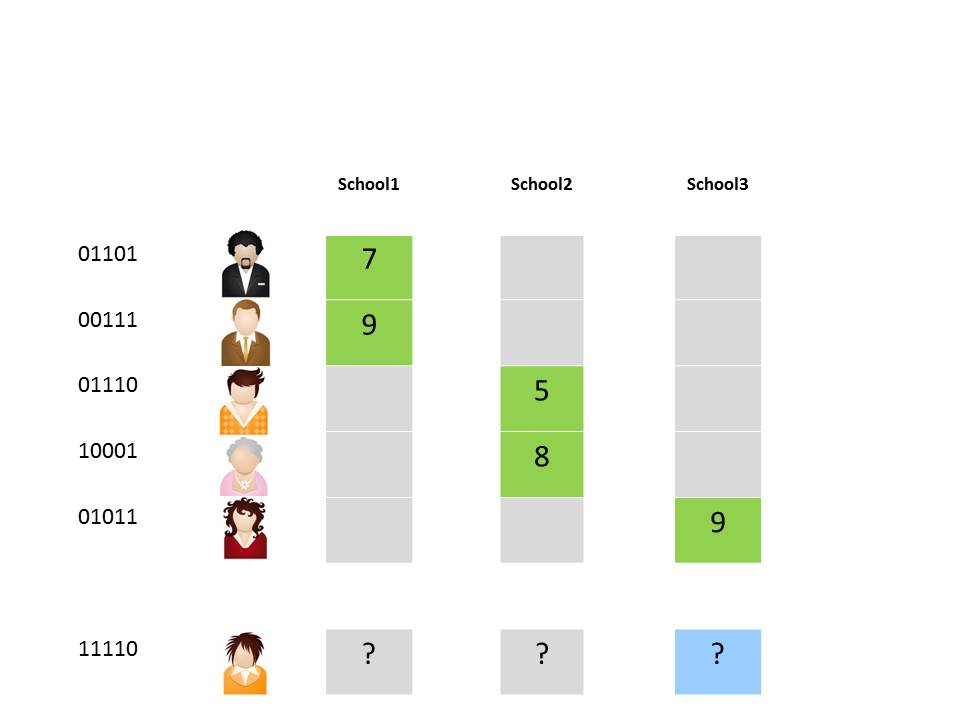
\includegraphics[width=0.9\textwidth,trim = 0 0 100 100,clip]{Figures/pictures/Slide3}
\end{frame}

%\begin{frame}{Conventional MTP settings}
%\begin{definition}[Label ranking] 
%A multi-label classification problem is a specific instantiation of the general framework, which exhibits the following additional properties: 
%\begin{enumerate}
%\item[P5.] The cardinality of $\mathcal{T}$ is $m$; this implies that all targets are observed during training. 
%\item[P6.] No side information is available for targets. Again, without loss of generality, we can hence identify targets with natural numbers, such that the target space is $\mathcal{T} = \{1,...,m\}$. 
%\item[P7.] The score matrix $Y$ has no missing values. 
%\item[P8c.] The score set is $\mathcal{Y} = \{1, \ldots , m\}$, and the scores (interpreted as ranks) are such that $y_{ij} \neq y_{ik}$ for all $1 \leq j,k \neq m$. 
%\end{enumerate}
%\end{definition}
%\end{frame}
%
%
%
%
%
%\begin{frame}{Conventional MTP settings}
%\begin{itemize}
%\item
%In \emph{label ranking}\footnote{E.H., J.\ F\"urnkranz, W.\ Cheng, K.\ Brinker. Label Ranking by Learning Pairwise Preferences, Artificial Intelligence, 172, 2008.}, each instance is associated with a ranking (total order) of the targets.
%\end{itemize}
%%\vspace{0.8cm}
%\begin{center}
%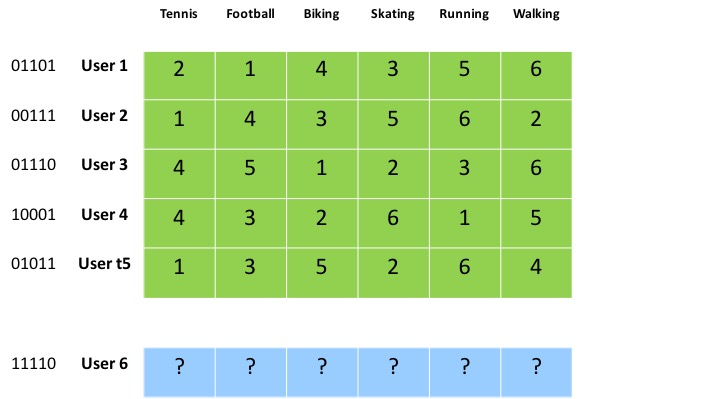
\includegraphics[width=0.8\textwidth]{Figures/pictures/labelranking}
%\end{center}
%\end{frame}





\begin{frame}{Let's assume a document hierarchy: \\
How would you call this machine learning problem?}
\begin{center}
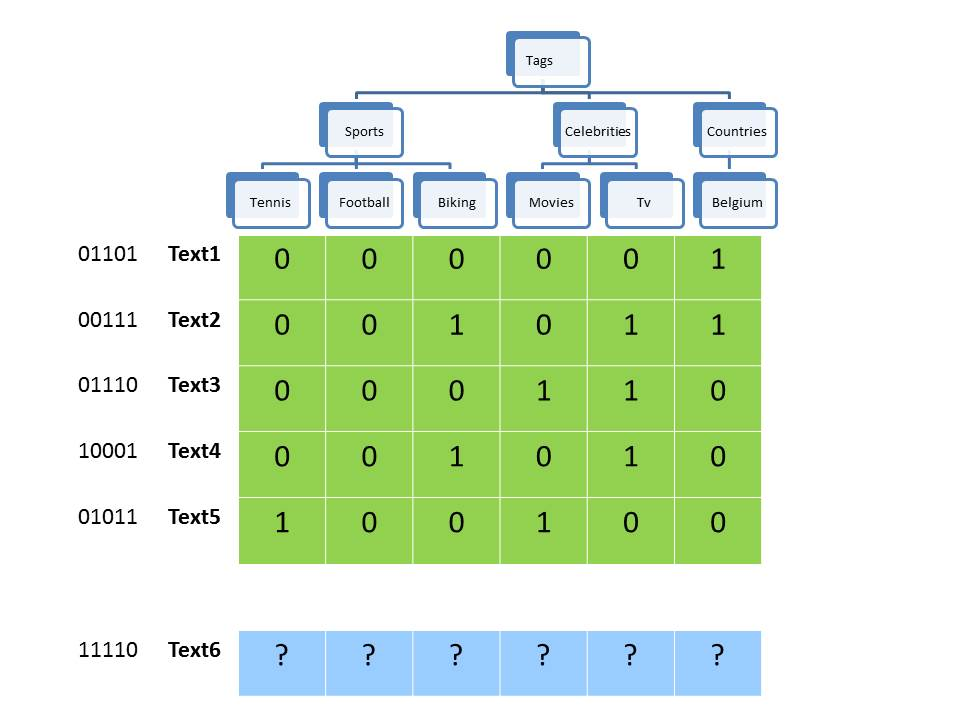
\includegraphics[width=0.75\textwidth,trim = 0 0 100 0,clip]{Figures/pictures/Slide5}
\end{center}
\end{frame}

\begin{frame}{Let's assume a target representation: \\
How would you call this machine learning problem?}
\vspace{0.8cm}
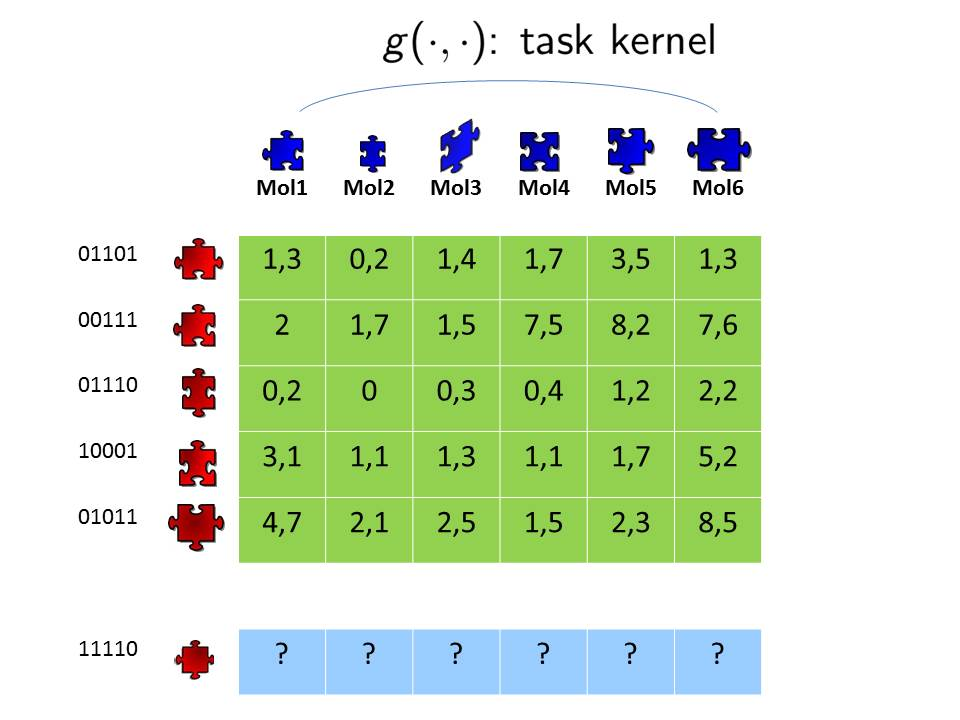
\includegraphics[width=0.9\textwidth,trim = 0 0 0 90,clip]{Figures/pictures/Slide4}

\end{frame}

\begin{frame}{Let's assume a target representation: \\
How would you call this machine learning problem?}
\begin{center}
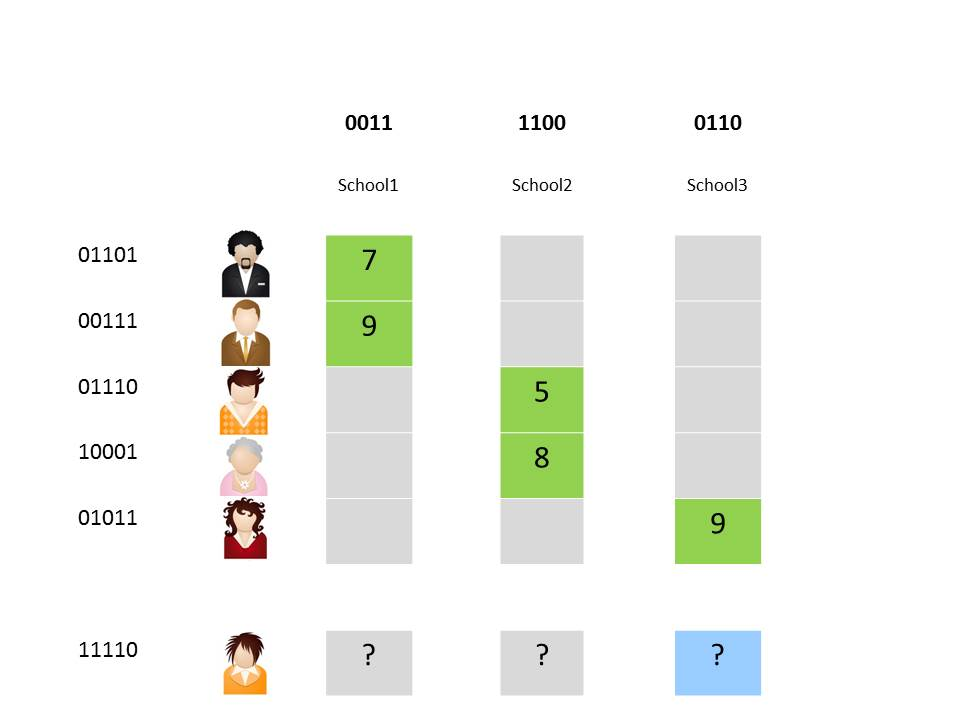
\includegraphics[width=0.8\textwidth,trim = 0 0 100 30,clip]{Figures/pictures/Slide6}
\end{center}

\end{frame}







\begin{frame}{Learning with side information on targets}
\begin{itemize}
\item Additional side information about the target space is available.
\item Examples: 
\begin{itemize}
\item Taxonomy on document categories (\emph{hierarchy}).
\item Representation for the target molecules in drug design application (\emph{structured representation}).
\item Information about schools and courses (geographical location, qualifications of the teachers, reputation of the school, etc.) in student mark forecasting application (\emph{feature representation}).
\end{itemize}
\item Such problems are often referred to as dyadic prediction, link prediction, or network inference settings.
\end{itemize}
\end{frame}
%
%
%\begin{frame}{Learning with side information on targets}
%\begin{itemize}
%\item
%Generally speaking, such settings cover problems that obey the four properties listed in the MTP definition. 
%\item Labels $y_{ij}$ can be arranged in a matrix $Y$, which is often sparse. 
%\item Thus, one may argue that \emph{dyadic prediction} is nothing else than \emph{multi-task learning with task features}. 
%\item However, MTP terminology is rarely used in the dyadic prediction literature. 
%\end{itemize}
%\end{frame}
%
%
%
%
%
%\begin{frame}{Inductive versus transductive learning problems}
%\begin{itemize} 
%\item In the previous problems, 
%\begin{itemize}
%\item predictions need be be generated for novel instances, 
%\item whereas the set of targets is known beforehand and observed during the training phase.
%\end{itemize}
%\item These problems are \emph{inductive} w.r.t.\ instances and \emph{transductive} w.r.t.\ targets.
%\item   
%\emph{Side information} is of crucial importance for generalizing to novel targets that are unobserved during the training phase.
%%such as a novel target molecule in the drug design example, a novel tag in the document annotation example, or a novel course in the student grading example. 
%\end{itemize}
%\end{frame}
%

\begin{frame}{Inductive versus transductive learning problems}
% voorbeeldje met boeken
%\vspace{0.6cm}
$$\qquad g(.,.): \mbox{target similarity}$$

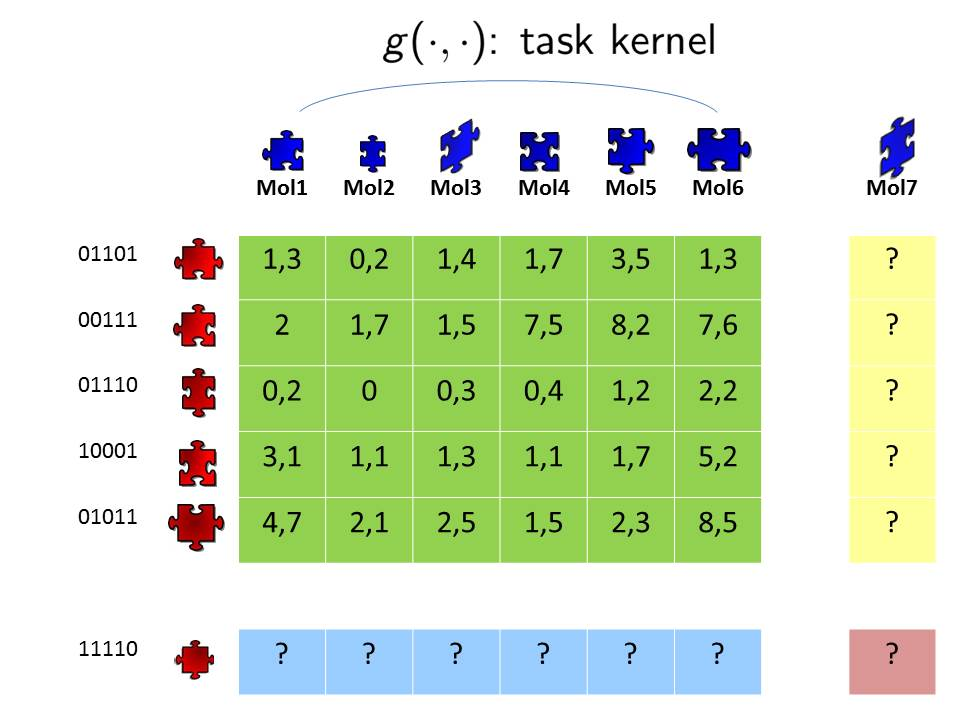
\includegraphics[width=0.9\textwidth,trim = 0 0 0 60,clip]{Figures/pictures/Slide7}
\end{frame}

\begin{frame}{Important subdivision of different learning settings}
   \center
	\vspace{0.4cm}
   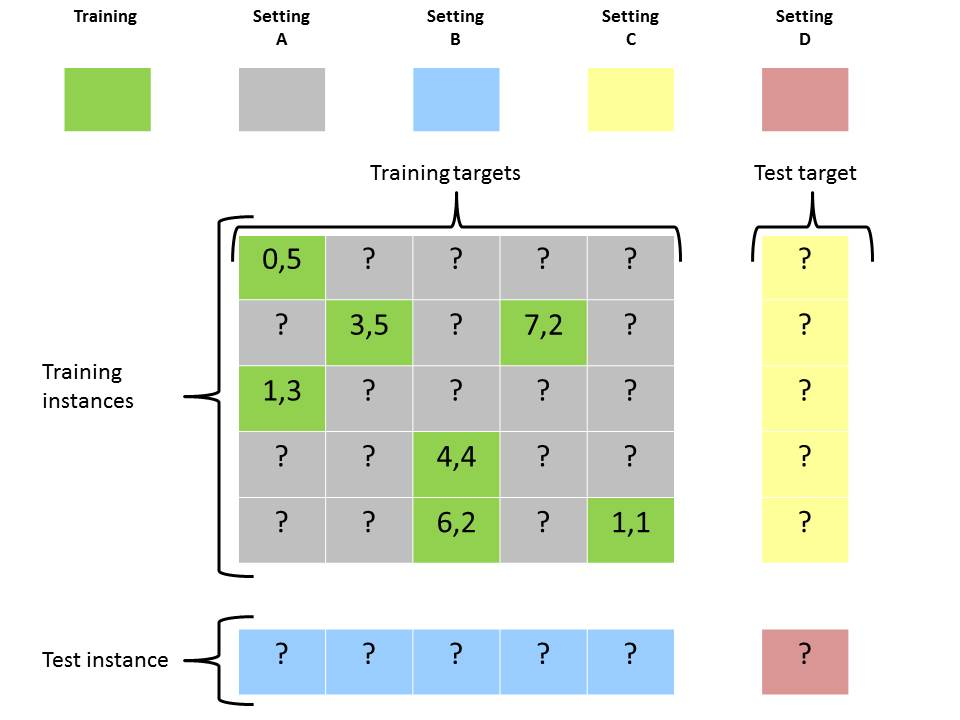
\includegraphics[width=0.9\textwidth]{Figures/pictures/Slide16} % requires the graphicx package
\end{frame}

%
%\begin{frame}{General framework}
%\begin{definition}[Multi-target prediction]
%A multi-target prediction setting is characterized by instances $\vec{x} \in \mathcal{X}$ and targets $\vec{t} \in \mathcal{T}$ with the following properties: 
%\begin{itemize} 
%\item[P1.] A training dataset $\mathcal{D}$ consists of triplets $(\vec{x}_i,\vec{t}_j,y_{ij})$, where $y_{ij} \in \mathcal{Y}$ denotes a score that characterizes the relationship between the instance $\vec{x}_i$ and the target $\vec{t}_j$.  
%\item[P2.] In total, $n$ different instances and $m$ different targets are observed during training, with $n$ and $m$ finite numbers. Thus, the scores $y_{ij}$ of the training data can be arranged in an $n \times m$ matrix $Y$, which is in general incomplete, i.e., $Y$ has missing values.
%\item[P3.] The score set $\mathcal{Y}$ is one-dimensional. It consists of nominal, ordinal or real values.  
%\item[P4.] The goal consists of predicting scores for any instance-target couple $(\vec{x},\vec{t}) \in \mathcal{X} \times \mathcal{T}$.   
%\end{itemize}
%\end{definition}
%
%\end{frame}
%
%
%
%
%\begin{frame}{Specific MTP settings: one example}
%\begin{definition}[Multivariate regression] 
%A multivariate regression problem is a specific instantiation of the general framework, which exhibits the following additional properties: 
%\begin{enumerate}
%\item[P5.] The cardinality of $\mathcal{T}$ is $m$. This implies that all targets are observed during training. 
%\item[P6.] No side information is available for targets. Without loss of generality, we can hence assign the numbers $1$ to $m$ as identifiers to targets, such that the target space is $\mathcal{T} = \{1,...,m\}$. 
%\item[P7.] The score matrix $Y$ has no missing values. 
%\item[P8.] The score set is $\mathcal{Y} = \mathbb{R}$. 
%\end{enumerate}
%\end{definition}
%\end{frame}





\begin{frame}{Inductive versus transductive learning problems}
\begin{definition}[Zero-shot learning]
A zero-shot learning problem is a specific instantiation of the general framework with the following additional property: 
\begin{enumerate}
\item[P5*.] $m < m^* = |\mathcal{T}|$. Some targets are hence not observed during training, but may nevertheless appear at prediction time.  
\end{enumerate}
\end{definition}
\pause

\begin{itemize}
\item By substituting P5 with P5*, one now tackles problems that are inductive instead of transductive w.r.t.\ targets. 
\item The same subdivision can be made for instances. 
\item In total, the four different settings referred to as A, B, C, D can be distinguished (in the presence of side information). %about instances and targets.
\item Theoretically, settings B and C are identical/symmetric, though there are practical differences/asymmetries. 
\end{itemize}
\end{frame}




\begin{frame}{Inductive versus transductive learning problems}
\begin{definition}[Matrix completion]
A matrix completion problem is a specific instantiation of the general framework with the following additional properties: 
\begin{enumerate}
\item[P5.] The cardinality of $\mathcal{T}$ is $m$. This implies that all targets are observed during training. 
\item[P6.] No side information is available for targets. Without loss of generality, we can hence assign identifiers to targets from the set $\{1,...,m\}$ such that the target space is $\mathcal{T} = \{1,...,m\}$.
\item[P9.] The cardinality of $\mathcal{X}$ is $n$. This implies that all instances are observed during training. 
\item[P10.] No side information is available for instances. Without loss of generality, we can hence assign identifiers to instances from the set $\{1,...,n\}$, such that the instance space is $\mathcal{X} = \{1,...,n\}$.
\end{enumerate}
\end{definition}
\end{frame}




\section{A unifying view on MTP methods}


\begin{frame}{Overview of this talk}

\tableofcontents

\end{frame}

\begin{frame}{A unifying view on MTP methods}

\begin{center}
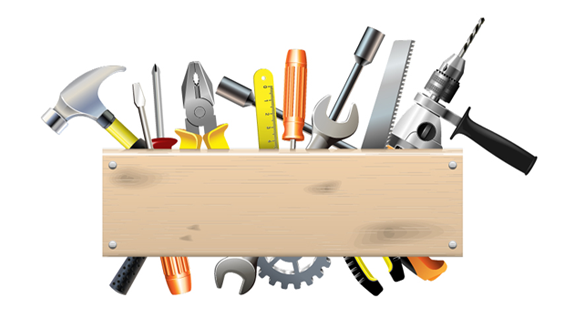
\includegraphics[scale=0.3]{pics/tools}

\begin{tabular}{ll}
\hline
Group of methods & Applicable setting \\
\hline
\hline
Independent models & B \\
Similarity-enforcing methods & B   \\ 
Relation-exploiting methods & B and D  \\
Relation-constructing methods & B \\
Representation-exploiting methods & B and D \\
Representation-constructing methods & A and B \\
\hline  
\end{tabular}
\end{center}
\end{frame}

%\begin{frame}{Different learning settings revisited}
   %\center
	%\vspace{0.4cm}
   %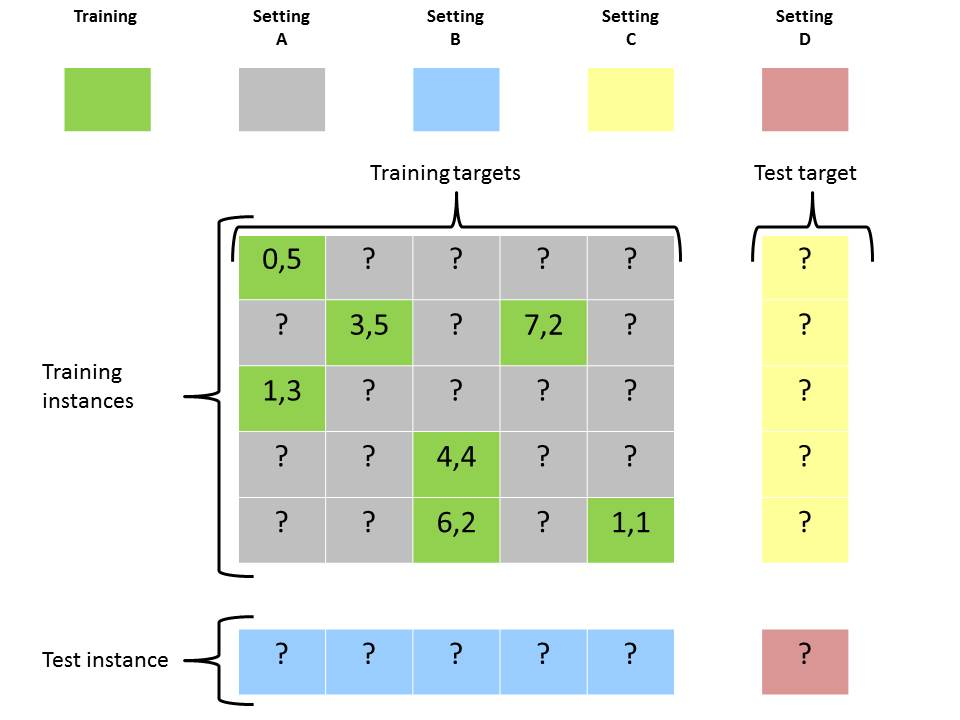
\includegraphics[width=0.9\textwidth]{Figures/pictures/Slide16} % requires the graphicx package
%\end{frame}


\begin{frame}{A baseline method:\\
learning a model for each target independently}
% voorbeeldje met boeken
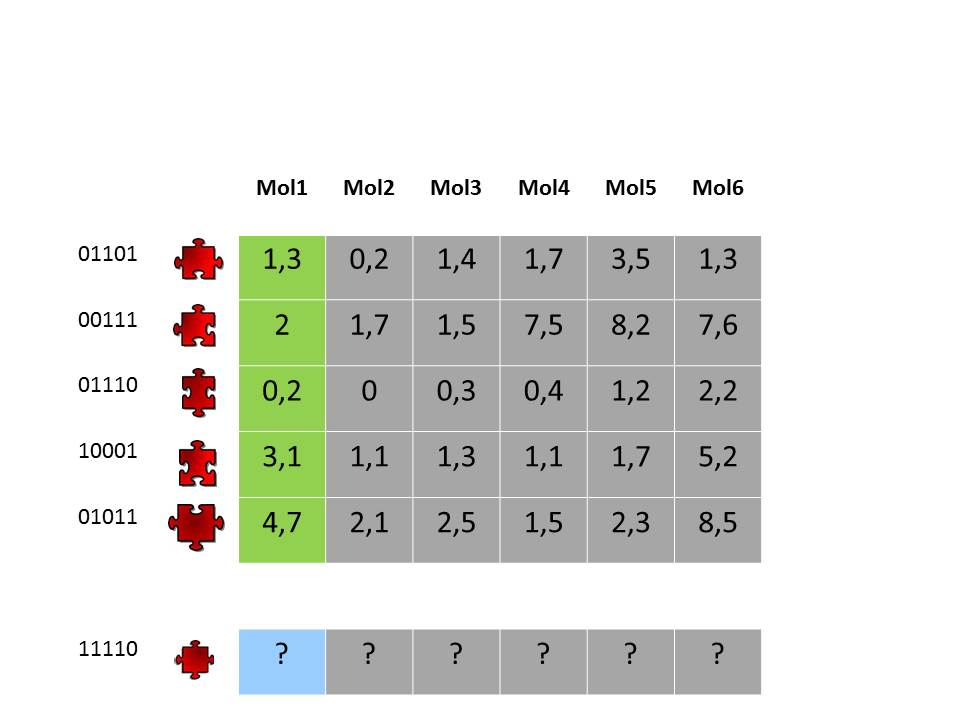
\includegraphics[width=0.9\textwidth,trim = 0 0 100 100,clip]{Figures/pictures/Slide13}
\end{frame}

\begin{frame}{A baseline method:\\
learning a model for each target independently}
% voorbeeldje met boeken
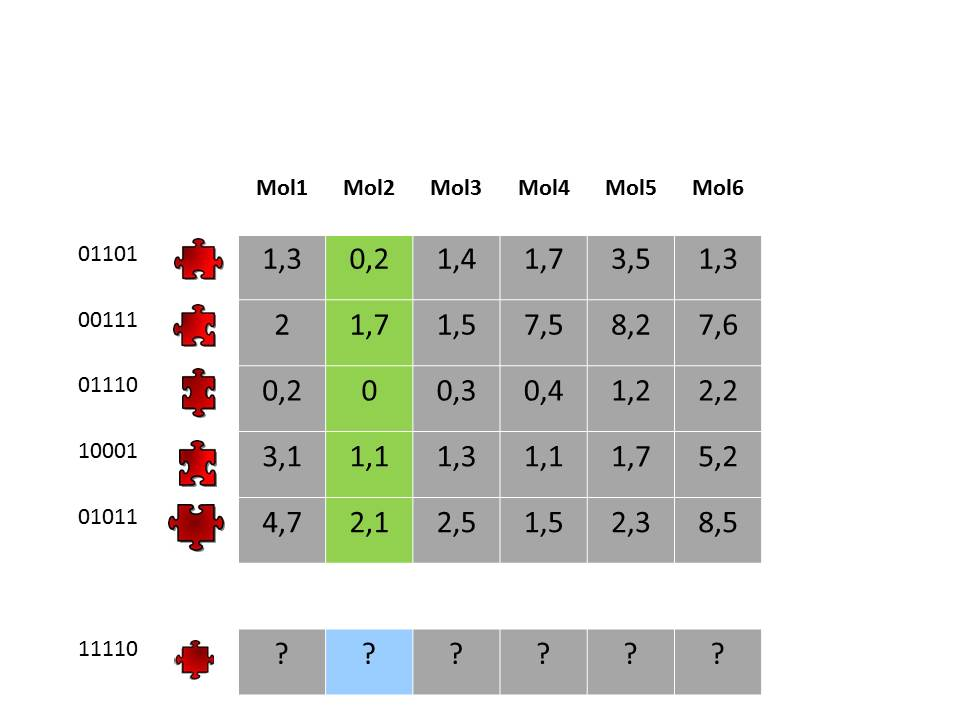
\includegraphics[width=0.9\textwidth,trim = 0 0 100 100,clip]{Figures/pictures/Slide14}
\end{frame}

\begin{frame}{A baseline: Independent Models}
% voorbeeldje met boeken
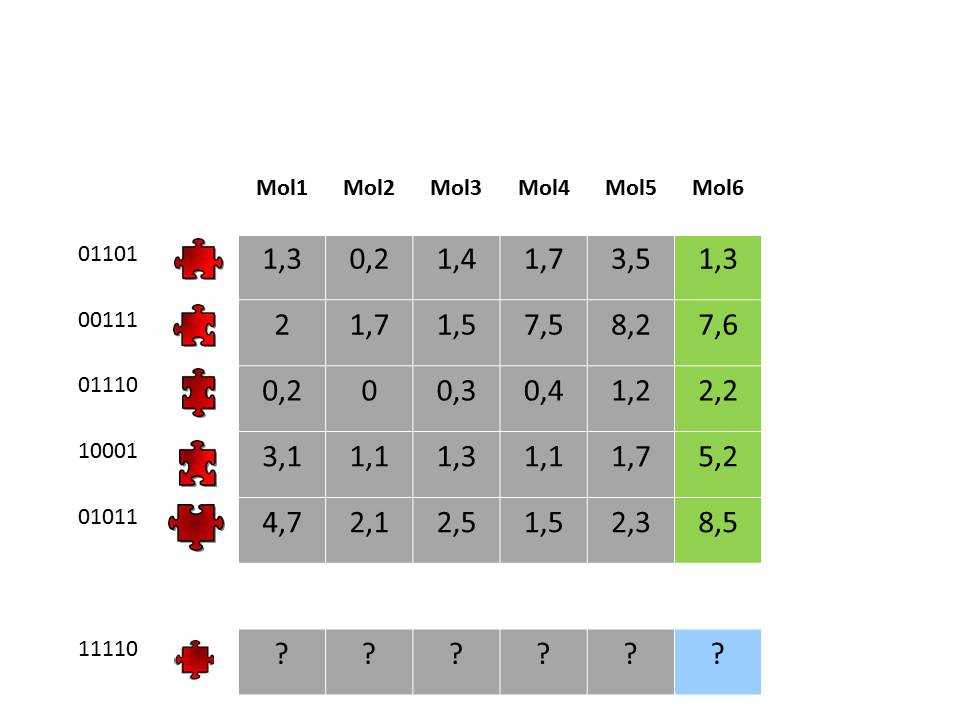
\includegraphics[width=0.9\textwidth,trim = 0 0 100 100,clip]{Figures/pictures/Slide15}
\end{frame}










\begin{frame}{Enforcing similarity in (Deep) Neural Networks}
\begin{center}
Commonly-used architecture: weight sharing among targets\footnote{Caruana, Multitask learning: A knowledge-based source of inductive bias. Machine
Learning 1997} \\
\vspace{0.2cm}
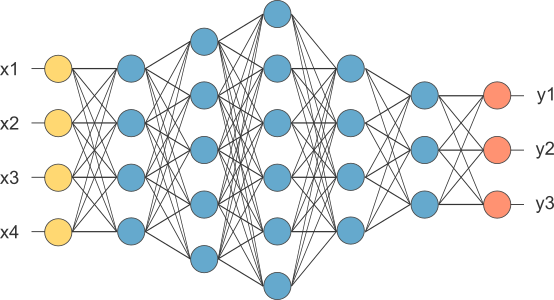
\includegraphics[scale=0.6]{Figures/weightsharing}
\end{center}
\end{frame}


\begin{frame}{Exploiting relations in regularization terms}

\begin{center}
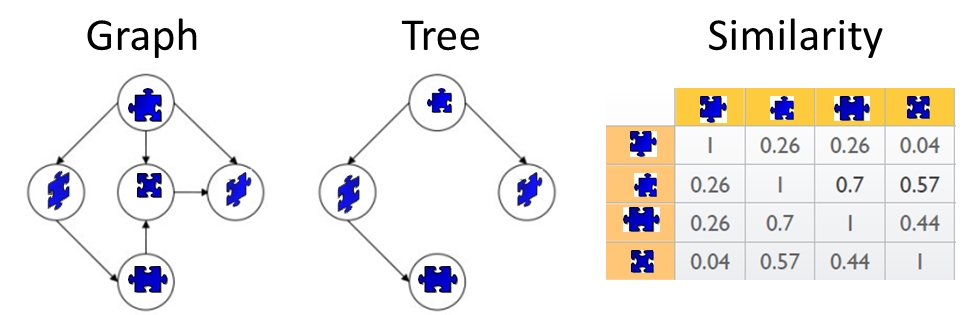
\includegraphics[width=\textwidth]{pics/targetrelations}
\end{center} \pause 

Graph-based regularization is an approach that can be applied to the three types of relations\footnote{Gopal and Yang, Recursive regularization for large-scale classification with hierarchical
and graphical dependencies, KDD 2013}: 
\begin{equation*}
\min_A ||Y - XA ||^2_F + \lambda \sum_{i=1}^m \sum_{j \in \mathcal{N}(i)} ||\vec{a}_i - \ \vec{a}_j||^2 
\end{equation*}

\end{frame}




\begin{frame}{Constructing target hierarchies}

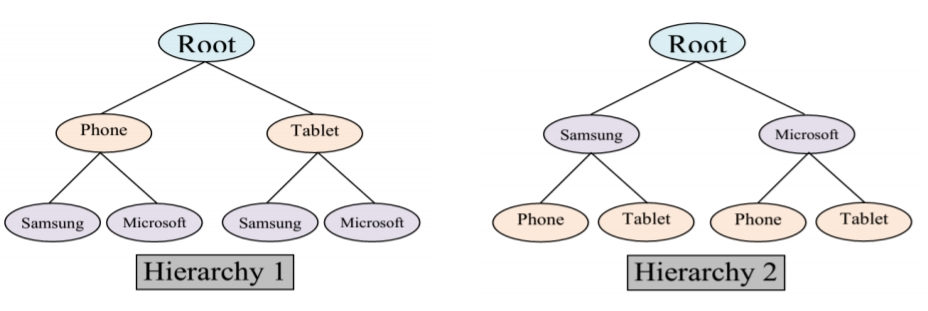
\includegraphics[width=\textwidth]{pics/hierarchies}

\begin{itemize}
\item It might be difficult for a human expert to define a hierarchy\footnote{Rangwala and Naik, Tutorial on Large-Scale Hierarchical Classification, KDD 2017.}
\item Perhaps one can try to learn the hierarchy from data? 
\item Algorithms: level flattening, node removal, hierarchy modification, hierarchy generation, etc.
\end{itemize}


\end{frame}

\begin{frame}{Learning target embeddings from text: Word2Vec}

Predict the probability of the next word $w_t$ given the previous words $h$\footnote{Mikolov et al., Efficient Estimation of Word Representations in
Vector Space, Arxiv 2013}:
$$P(w_t \given h) = \frac{\exp(f(w_t,h))}{\sum_{\mathrm{all words}} \exp(f(w_t,h))}$$
\begin{columns}
\begin{column}{5cm}
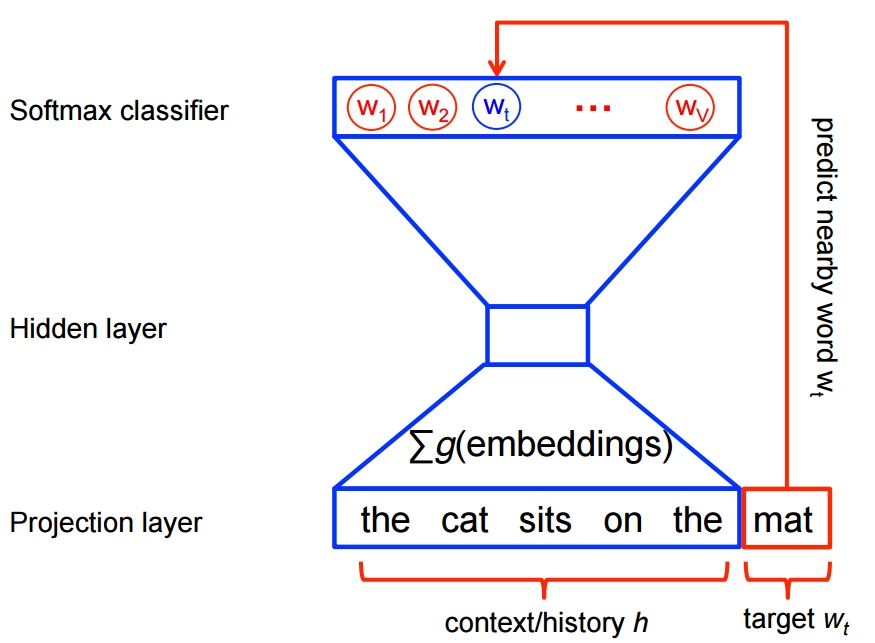
\includegraphics[scale=0.2]{Figures/word2vec}
\end{column}
\begin{column}{6cm}
\hspace{1cm} 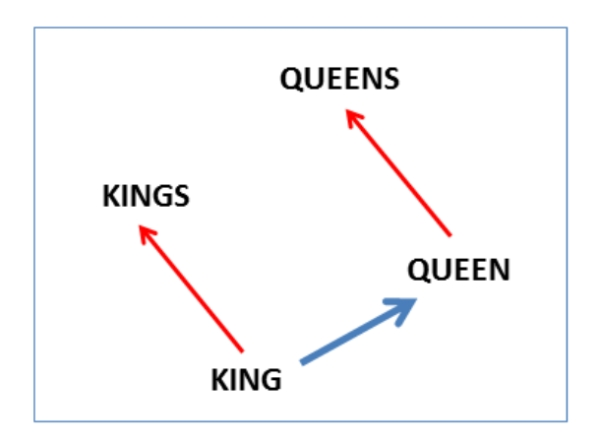
\includegraphics[scale=0.2]{Figures/kingqueen}
\end{column}
\end{columns}



\end{frame}



\begin{frame}{Low-rank approximation in Setting A}

Factorize the matrix $Y$ instead of the parameter matrix $A$: 
\begin{center}
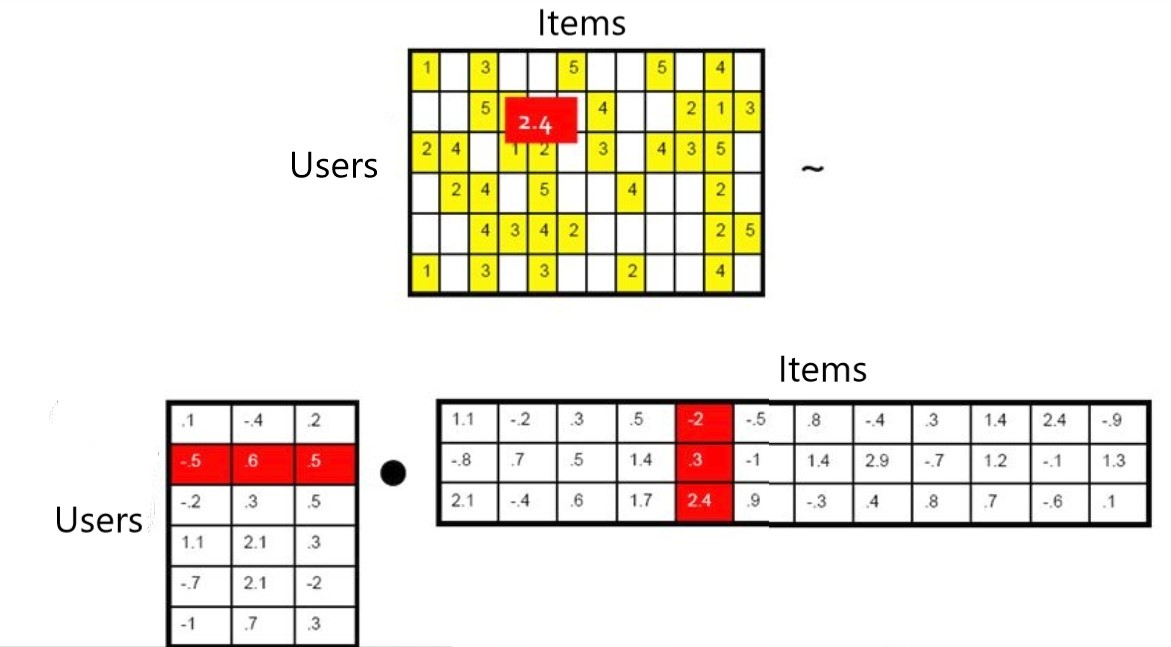
\includegraphics[width=11cm]{Figures/matrixcompletion2}
\end{center}
$$Y \qquad = \qquad  U \qquad \times \qquad V \qquad $$

\end{frame}





\begin{frame}{Conclusions and further reading}

\begin{itemize}
\item Multi-target prediction is an active field of research that connects different types of machine learning problems
\item In the corresponding subfields of machine learning, problems have typically been solved in isolation, without establishing connections between methods
\item When analyzing MTP methods, it is important to understand several concepts, such as the influence of loss functions, and the availability and absence of side knowledge
\end{itemize}

\begin{center}
{\bf Accompanying paper: \\
Waegeman et al. \\ Multi-Target Prediction: \\ A Unifying View on Problems and Methods} \\
Data Mining and Knowledge Discovery, 2019. 

\end{center}

\end{frame}


\begin{frame}{Questions? Remarks?}
\end{frame}

\section{Auto MTP: An automated multi-target prediction software package}

\begin{frame}{Overview of this talk}

\tableofcontents

\end{frame}

\begin{frame}{Automating the MTP framework (AutoMTP)}

 \begin{center}
 AutoMTP, an automated framework that performs setting selection and trains a model in an end-to-end approach.
 \end{center}
 
\begin{itemize}
\item[1.] A rule-based system for the algorithm selection step that is based on a custom-made questionnaire.
\item[2.] A flexible neural network architecture that can be used for the several subfields of MTP.
\end{itemize}


\end{frame}

\begin{frame}{Setting selection in Multi-Target Prediction}
\begin{center}
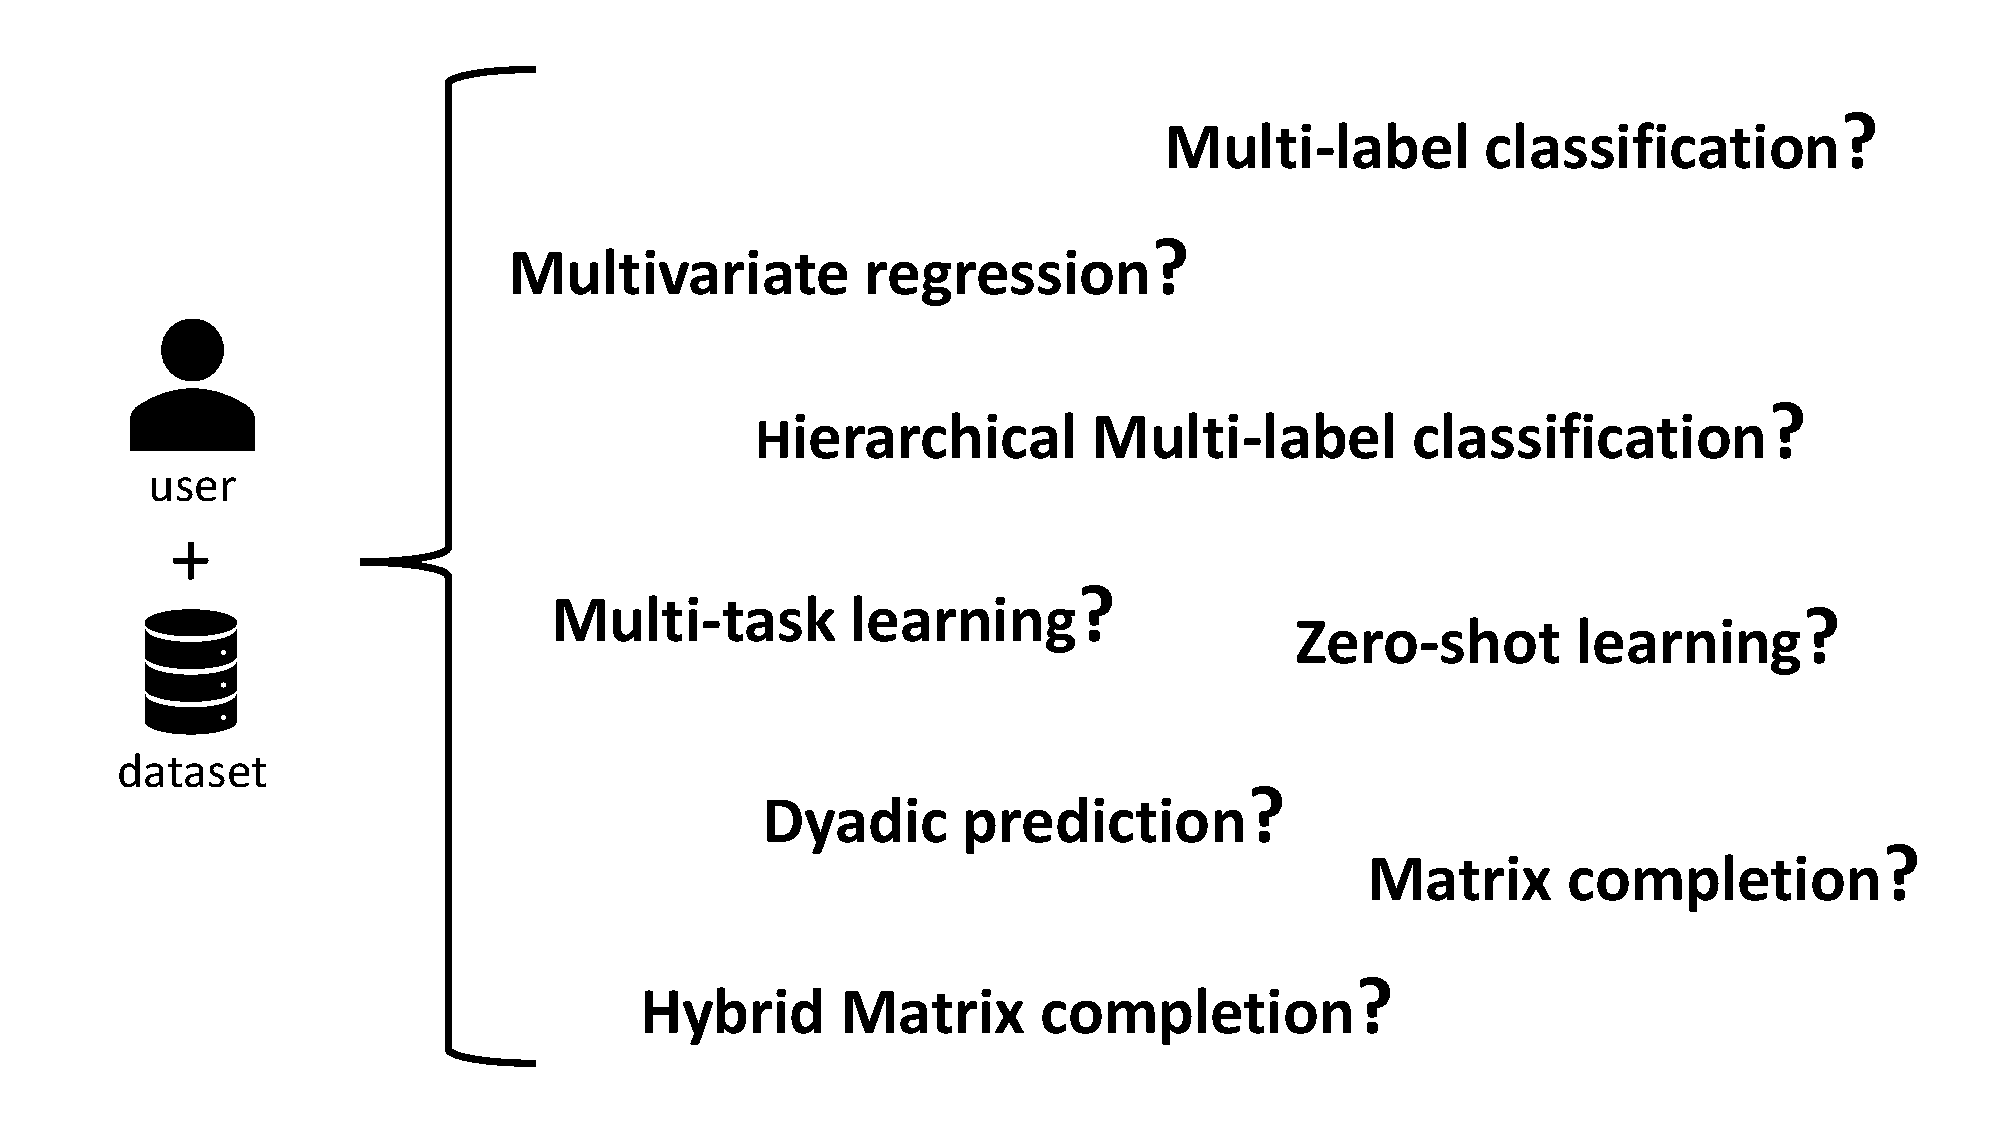
\includegraphics[width=\textwidth]{Dimitris_figures/MTPchoices.pdf}
\end{center}
\end{frame}

\begin{frame}{Purpose-made questionnaire}
\begin{itemize}
\itemindent=8pt    \item [\textbf{Q1}:] Is it expected to encounter novel instances during testing? \textbf{(yes/no)}
\itemindent=8pt    \item [\textbf{Q2}:] Is it expected to encounter novel targets during testing? \textbf{(yes/no)}
\itemindent=8pt    \item [\textbf{Q3}:] Is there side information available for the instances? \textbf{(yes/no)}
\itemindent=8pt    \item [\textbf{Q4}:] Is there side information available for the targets? \textbf{(yes/no)}
\itemindent=8pt    \item [\textbf{Q5}:] Is the score matrix fully observed? \textbf{(yes/no)}
\itemindent=8pt    \item [\textbf{Q6}:] What is the type of the target variable? \textbf{(binary/nominal/ordinal/real-valued)}
\end{itemize}
\end{frame}

\begin{frame}
{Multi-label classification (document categorization)}

\begin{columns}

\begin{column}{9cm}
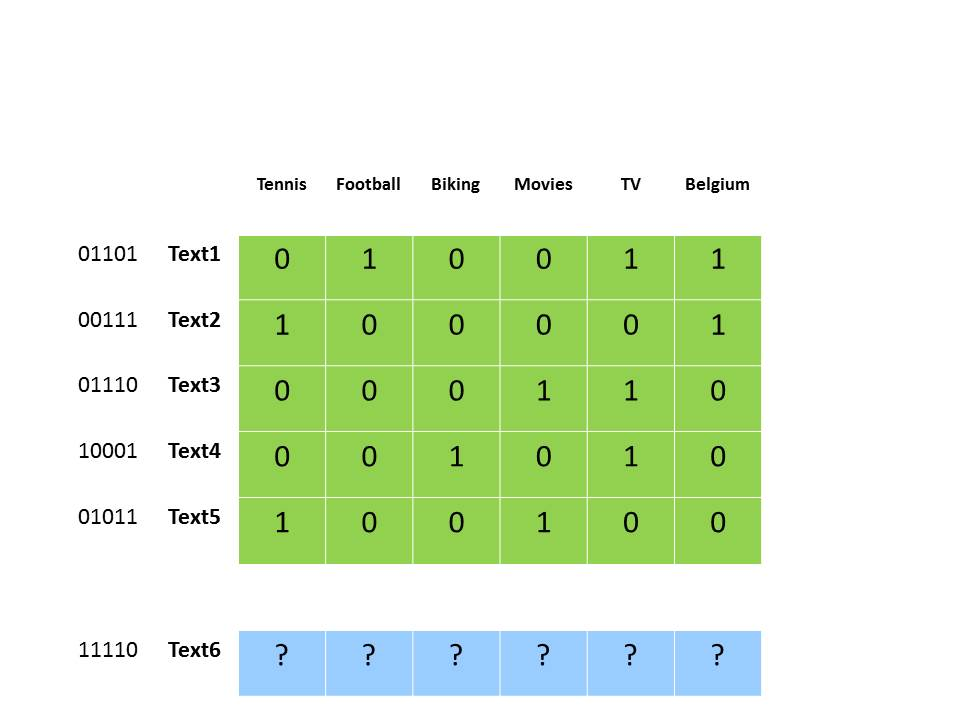
\includegraphics[width=0.9\textwidth,trim = 0 0 100 100,clip]{Figures/pictures/Slide2}
\end{column}

\begin{column}{7cm}
\begin{itemize}
\itemindent=2pt    \item [\textbf{Q1}:] \textbf{yes}
\itemindent=2pt    \item [\textbf{Q2}:] \textbf{no}
\itemindent=2pt    \item [\textbf{Q3}:] \textbf{yes}
\itemindent=2pt    \item [\textbf{Q4}:] \textbf{no}
\itemindent=2pt    \item [\textbf{Q5}:] \textbf{yes}
\itemindent=2pt    \item [\textbf{Q6}:]  \textbf{binary}
\end{itemize}
\end{column}

\end{columns}
\end{frame}



\begin{frame}
{Multi-label classification (image tagging)}

\begin{columns}

\begin{column}{9cm}
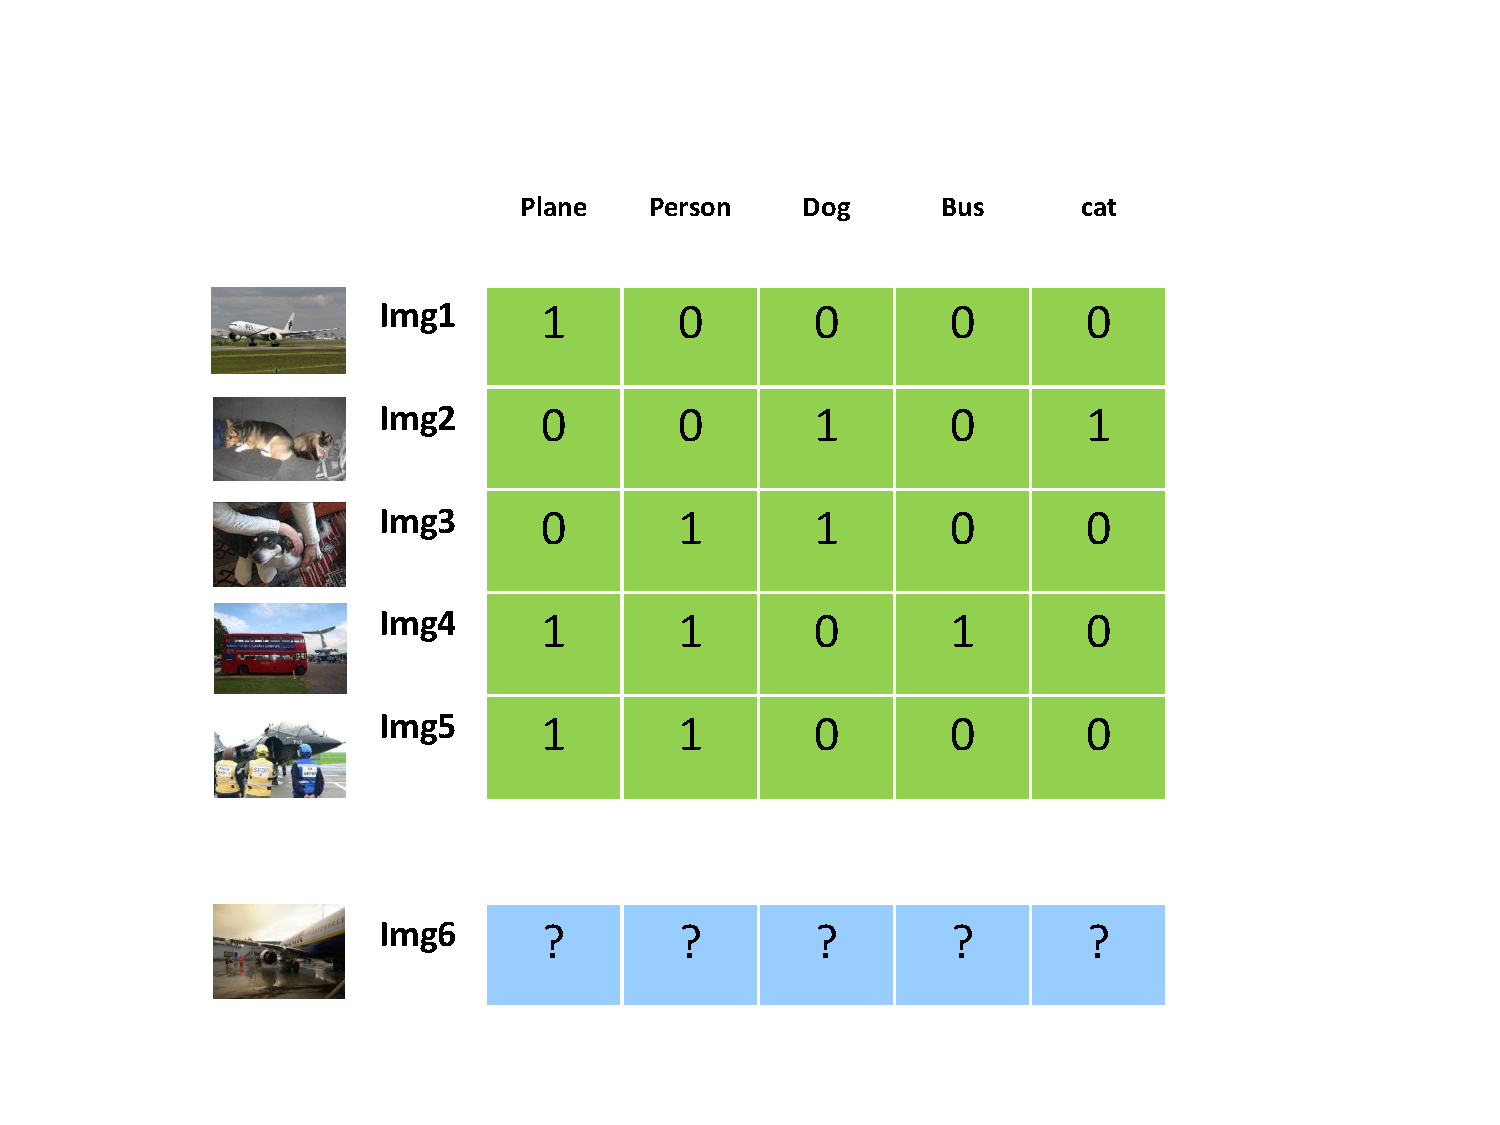
\includegraphics[width=0.9\textwidth,trim = 0 0 100 60,clip]{Dimitris_figures/MLC_image_classfication2.pdf}
\end{column}

\begin{column}{7cm}
\begin{itemize}
\itemindent=2pt    \item [\textbf{Q1}:] \textbf{yes}
\itemindent=2pt    \item [\textbf{Q2}:] \textbf{no}
\itemindent=2pt    \item [\textbf{Q3}:] \textbf{yes}
\itemindent=2pt    \item [\textbf{Q4}:] \textbf{no}
\itemindent=2pt    \item [\textbf{Q5}:] \textbf{yes}
\itemindent=2pt    \item [\textbf{Q6}:]  \textbf{binary}
\end{itemize}
\end{column}

\end{columns}
\end{frame}


\begin{frame}
{Multivariate regression (protein-ligand interaction prediction)}

\begin{columns}

\begin{column}{9cm}
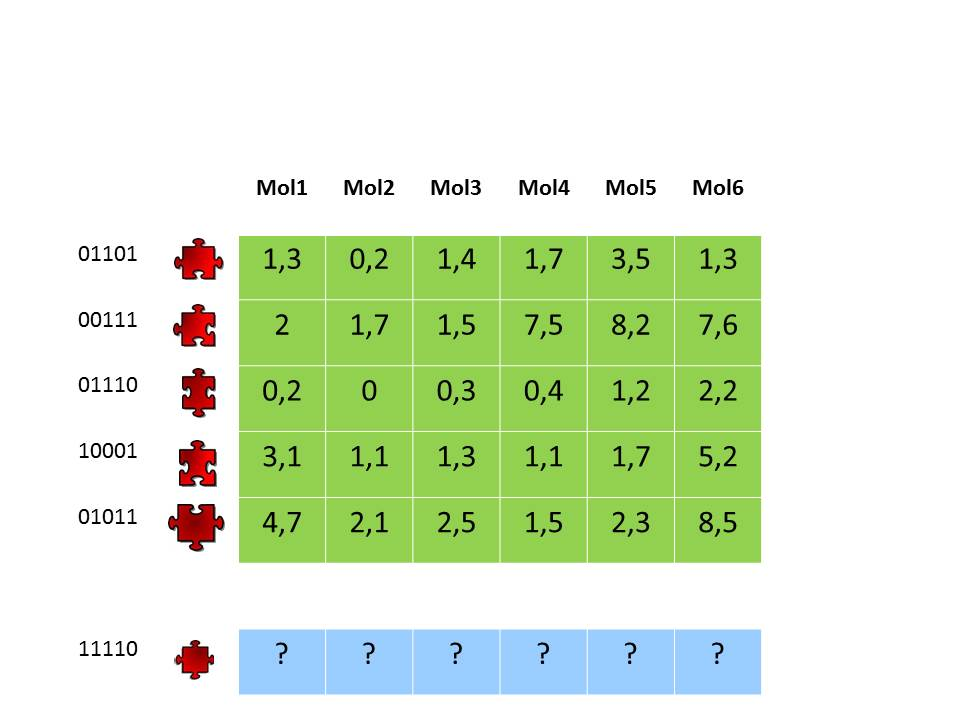
\includegraphics[width=0.9\textwidth,trim = 0 0 100 100,clip]{Figures/pictures/Slide1}
\end{column}

\begin{column}{7cm}
\begin{itemize}
\itemindent=2pt    \item [\textbf{Q1}:] \textbf{yes}
\itemindent=2pt    \item [\textbf{Q2}:] \textbf{no}
\itemindent=2pt    \item [\textbf{Q3}:] \textbf{yes}
\itemindent=2pt    \item [\textbf{Q4}:] \textbf{no}
\itemindent=2pt    \item [\textbf{Q5}:] \textbf{yes}
\itemindent=2pt    \item [\textbf{Q6}:]  \textbf{\color{red}real-valued}
\end{itemize}
\end{column}

\end{columns}
\end{frame}



\begin{frame}
{Multi-task Learning (predicting student marks)}

\begin{columns}

\begin{column}{9cm}
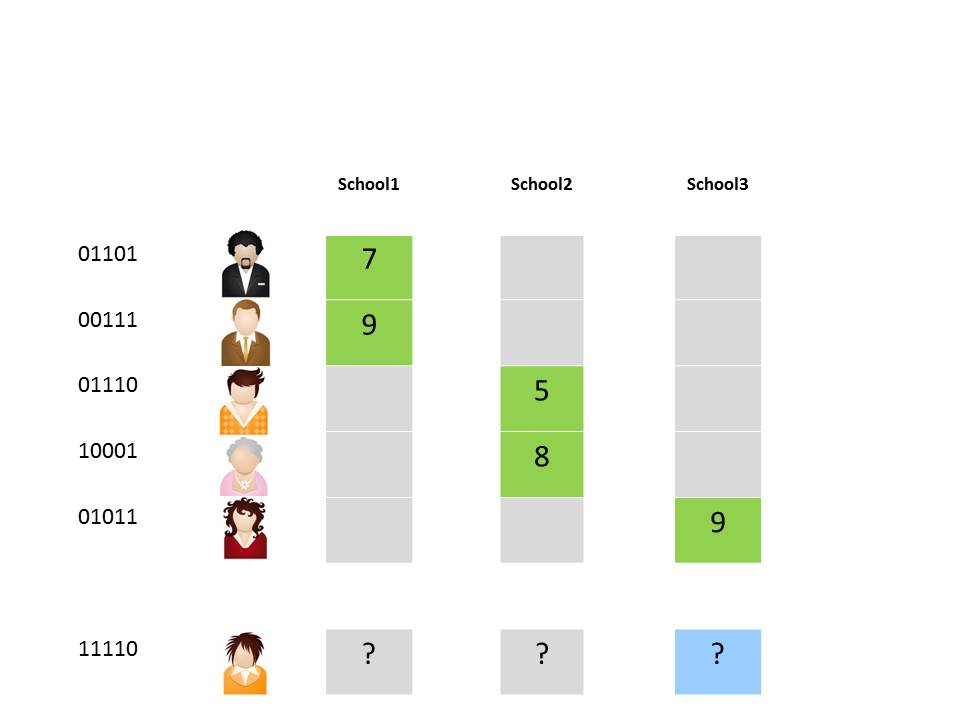
\includegraphics[width=0.9\textwidth,trim = 0 0 100 100,clip]{Figures/pictures/Slide3}
\end{column}

\begin{column}{7cm}
\begin{itemize}
\itemindent=2pt    \item [\textbf{Q1}:] \textbf{yes}
\itemindent=2pt    \item [\textbf{Q2}:] \textbf{no}
\itemindent=2pt    \item [\textbf{Q3}:] \textbf{yes}
\itemindent=2pt    \item [\textbf{Q4}:] \textbf{no}
\itemindent=2pt    \item [\textbf{Q5}:] \textbf{\color{red}no}
\itemindent=2pt    \item [\textbf{Q6}:]  \textbf{binary/\\real-valued}
\end{itemize}
\end{column}

\end{columns}
\end{frame}



\begin{frame}
{Dyadic prediction (protein-ligand interaction prediction)}

\begin{columns}

\begin{column}{9cm}
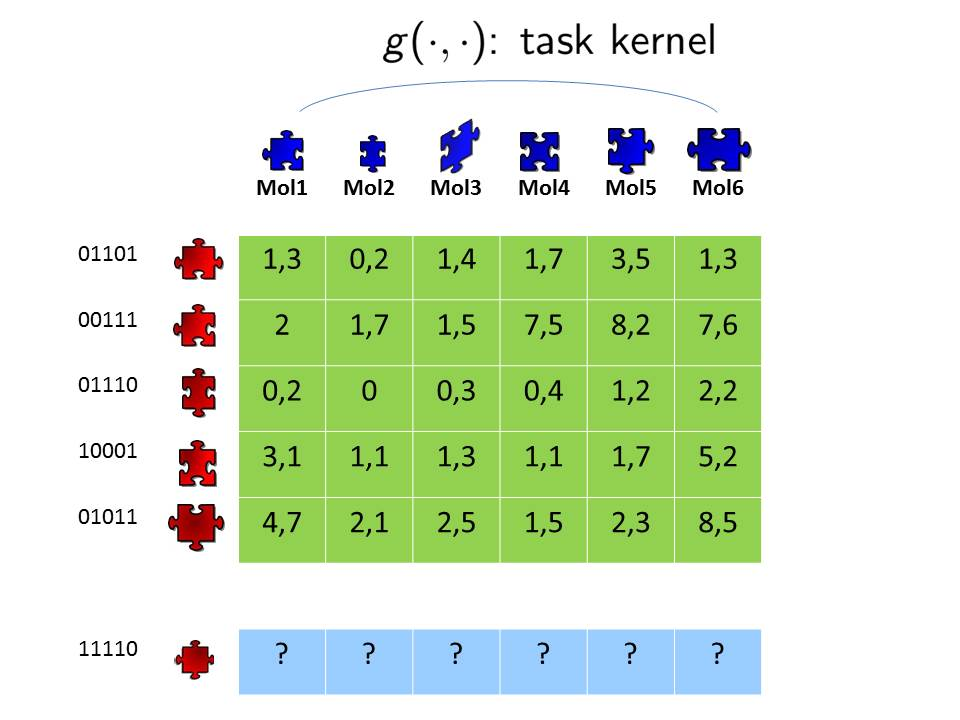
\includegraphics[width=0.9\textwidth,trim = 0 0 100 100,clip]{Figures/pictures/Slide4}
\end{column}

\begin{column}{7cm}
\begin{itemize}
\itemindent=2pt    \item [\textbf{Q1}:] \textbf{yes}
\itemindent=2pt    \item [\textbf{Q2}:] \textbf{no}
\itemindent=2pt    \item [\textbf{Q3}:] \textbf{yes}
\itemindent=2pt    \item [\textbf{Q4}:] \textbf{\color{red}yes}
\itemindent=2pt    \item [\textbf{Q5}:] \textbf{no}
\itemindent=2pt    \item [\textbf{Q6}:]  \textbf{binary/\\real-valued}
\end{itemize}
\end{column}

\end{columns}
\end{frame}



\begin{frame}
{Matrix Completion (Content recommendation)}

\begin{columns}

\begin{column}{9cm}
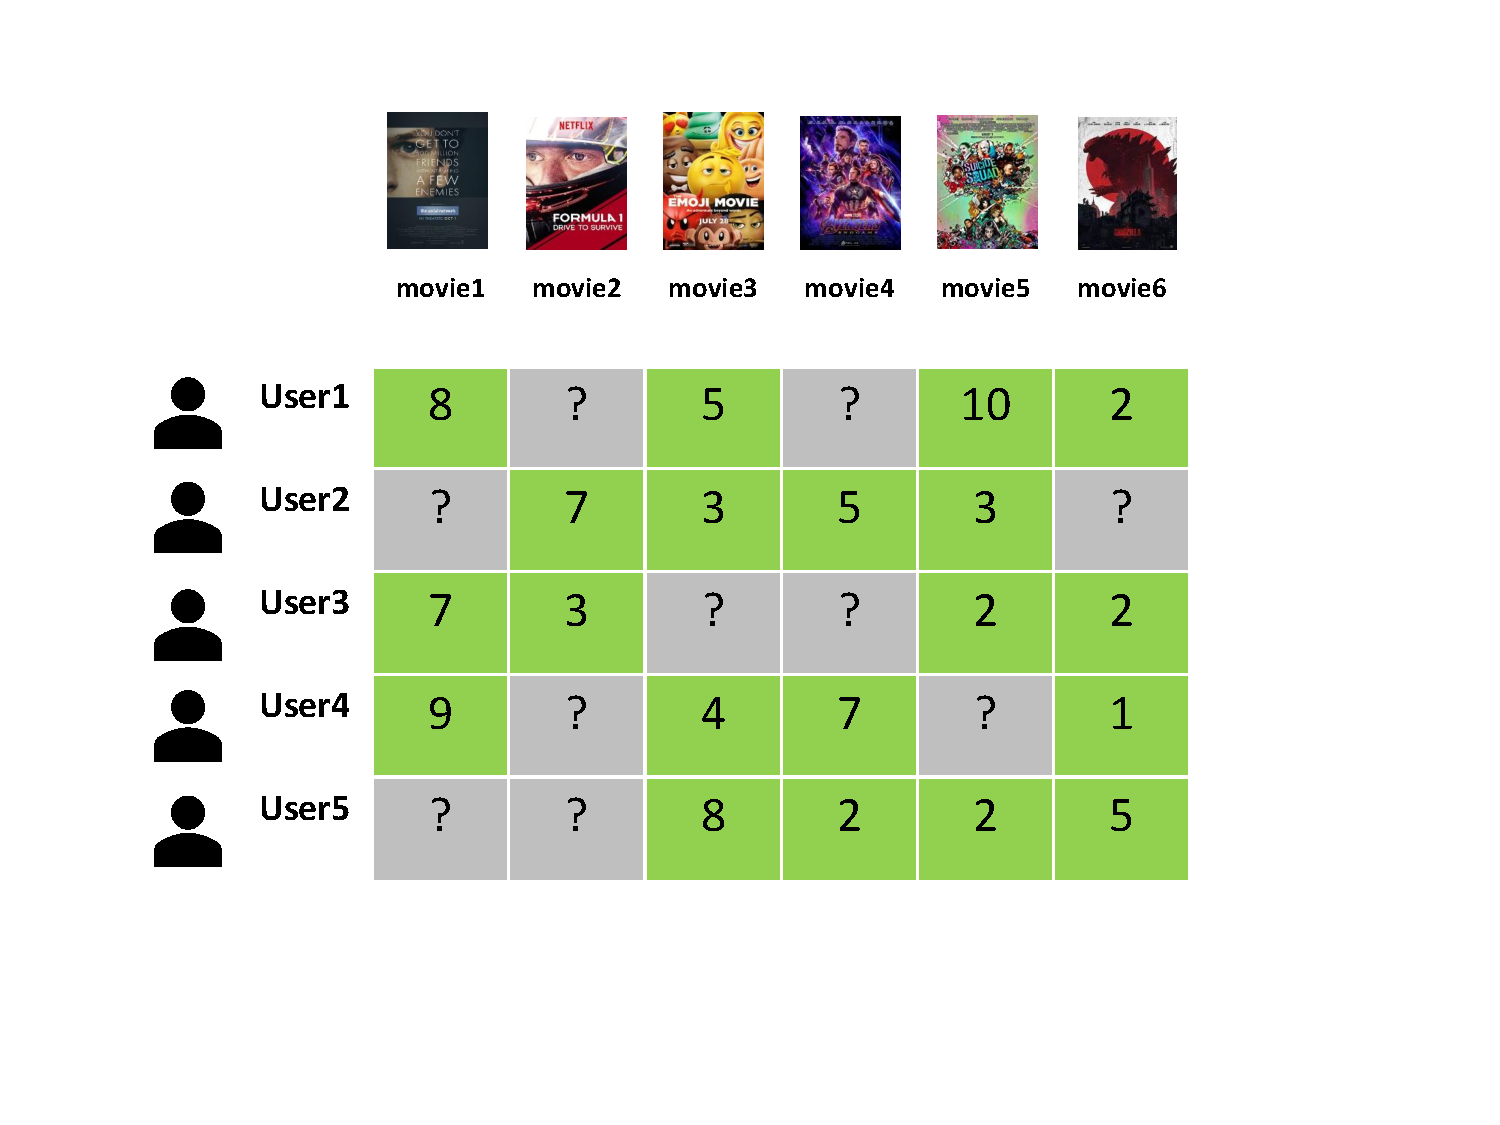
\includegraphics[width=0.9\textwidth,trim = 0 0 100 0,clip]{Dimitris_figures/MC_movie_recommendation.pdf}
\end{column}

\begin{column}{7cm}
\begin{itemize}
\itemindent=2pt    \item [\textbf{Q1}:] \textbf{no}
\itemindent=2pt    \item [\textbf{Q2}:] \textbf{no}
\itemindent=2pt    \item [\textbf{Q3}:] \textbf{no}
\itemindent=2pt    \item [\textbf{Q4}:] \textbf{no}
\itemindent=2pt    \item [\textbf{Q5}:] \textbf{no}
\itemindent=2pt    \item [\textbf{Q6}:]  \textbf{binary/\\real-valued}
\end{itemize}
\end{column}

\end{columns}
\end{frame}


\begin{frame}{Setting selection in Multi-Target Prediction}
\begin{table}[]
\centering
    \resizebox{\linewidth}{!}{
    \begin{tabular}{c|c|c|c|c|c|c}
    \textbf{Q1} & \textbf{Q2} & \textbf{Q3} & \textbf{Q4} & \textbf{Q5} & \textbf{Q6} & \textbf{MTP method}        \\
    \hline
    yes         & no          & yes         & no          & yes         & binary      & Multi-label classification\\
    yes         & no          & yes         & no          & yes         & real-valued & Multivariate regression\\
    yes         & no          & yes         & no          & no          & -           & Multi-task learning        \\
    yes         & no          & yes         & yes (hierarchy)   & yes         & binary      & Hierarchical Multi-label classification\\
    yes         & no          & yes         & yes         & no          & -           & Dyadic prediction\\
    yes         & yes         & yes         & yes         & no           & -           & Zero-shot learning\\
    no          & no          & no          & no          & no          & -           & Matrix completion\\
    no         & no         & yes           & yes           & no          & -           & Hybrid Matrix
    completion\\
    yes        & yes         & yes          & yes           & no        &  -           & Cold-start Collaborative filtering
    \end{tabular}}
\end{table}

\begin{itemize}
\item These questions generate 128 different combinations
\item Most of them lead to impossible tasks
\item \textbf{Simple rule:} generalization to novel drugs or targets necessitates the corresponding side information.
\end{itemize}

\end{frame}



\begin{frame}{A flexible neural network architecture}

First popularized by the neural  collaborative  filtering  (NCF)\footnote{ He, X., Liao, L., Zhang, H., Nie, L., Hu, X., Chua, T.S.: Neural collaborative filtering.In: Proceedings of the 26th International Conference on World Wide Web, pp. 173–182(2017)}  method  in  the  field  of  recommender systems

\begin{center}
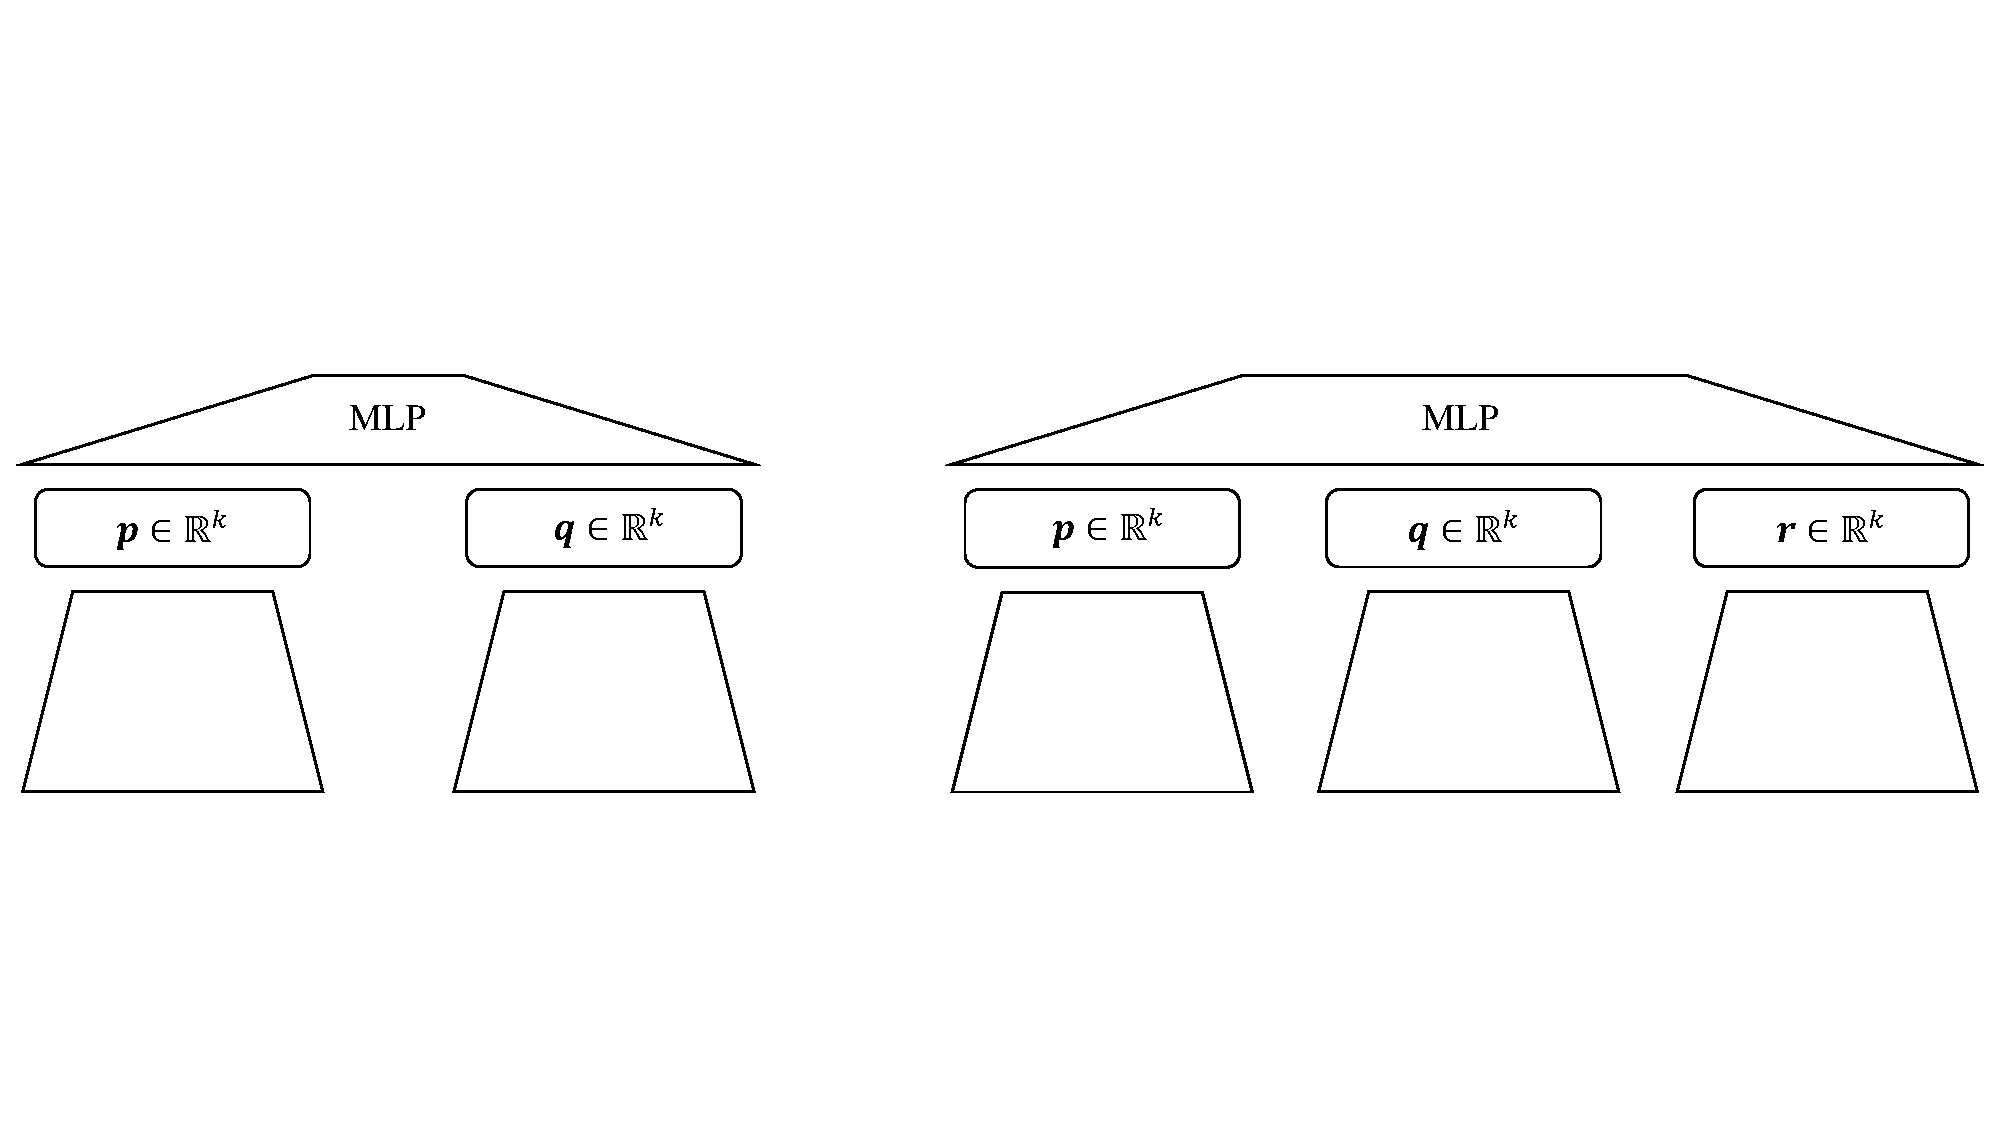
\includegraphics[width=0.9\textwidth,trim = 0 160 0 170,clip]{Dimitris_figures/dual_triple_branch_architecture.pdf}
\end{center}
 
The multi-branch architecture has two versions:
\begin{itemize}
\item[1.] The dual-branch architecture has to input branches (instances and targets).
\item[2.] The tri-branch architecture adds a third input for any available dynamic side information.
\end{itemize}

\end{frame}


\begin{frame}{A flexible neural network architecture 2}

Depending on the availability of side information:
\begin{itemize}
\item[1.] If side information is available: use it... 
\item[2.] If side information is missing: create one-hot encoded vectors.
\end{itemize}


\begin{center}
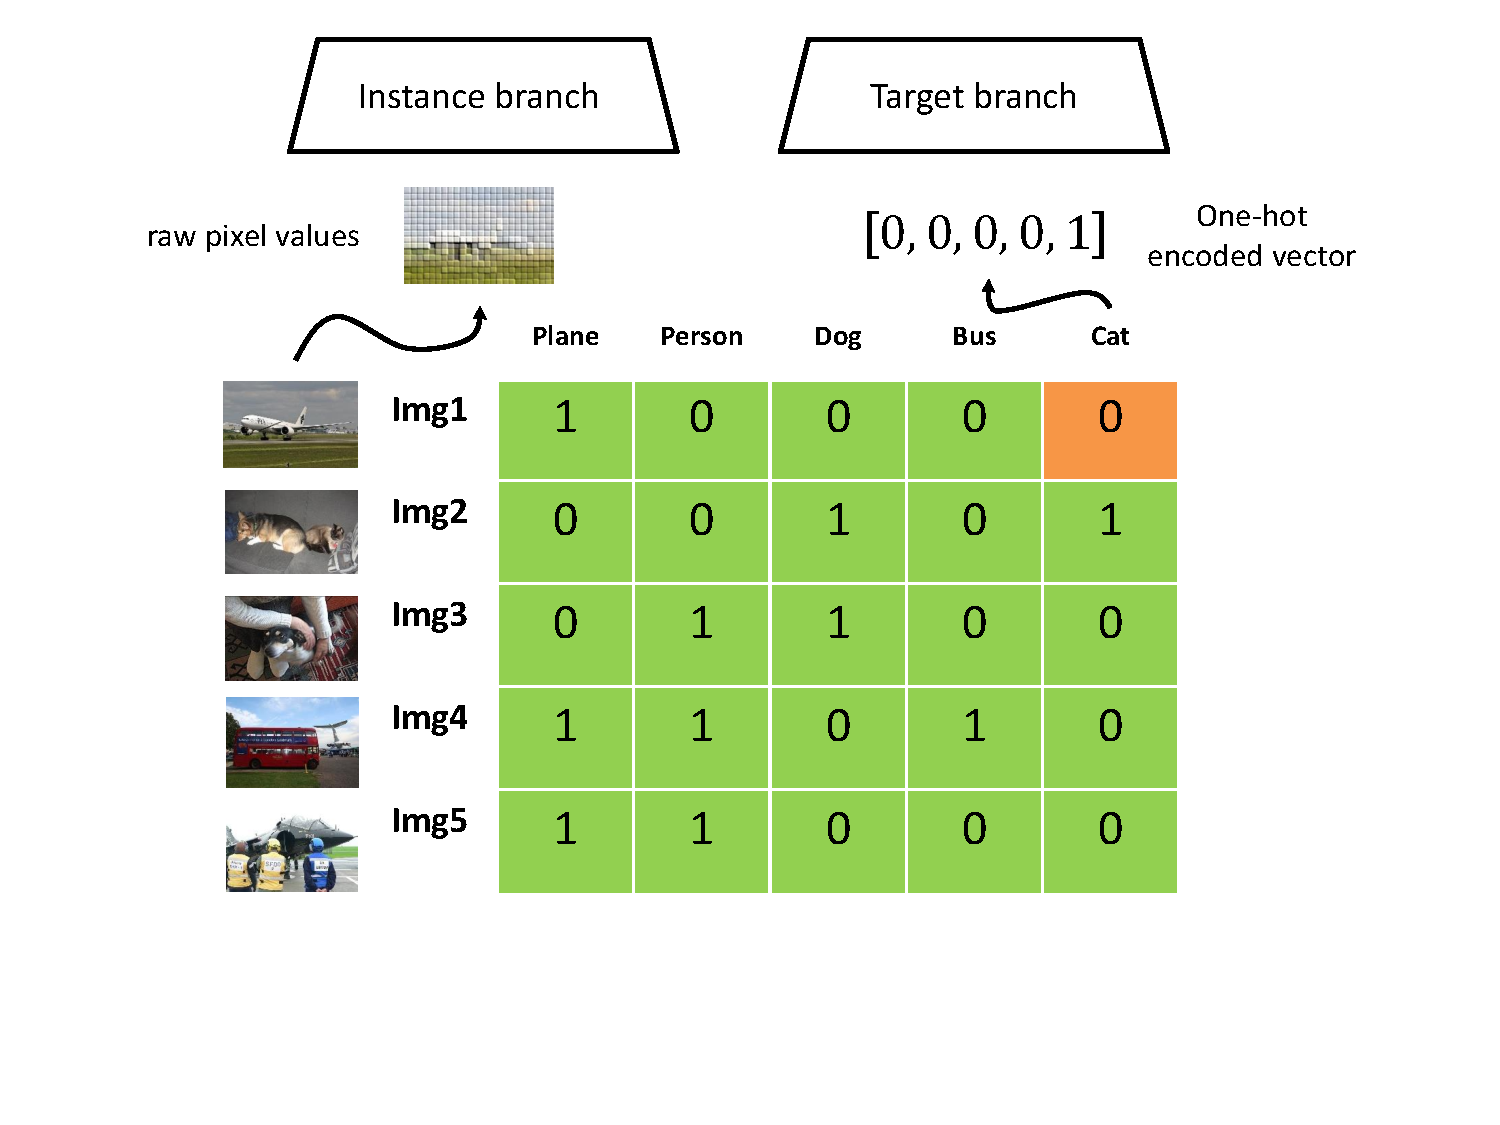
\includegraphics[width=0.9\textwidth,trim = 0 100 0 0,clip]{Dimitris_figures/regular_one_hot_inputs_example.pdf}
\end{center}

\end{frame}


\begin{frame}{A flexible neural network architecture 3}

 
Depending on the type of side information
\begin{itemize}
\item[1.] tabular data: fully connected layers.
\item[2.] images: convolutional neural network.
\item[3.] time-series: RNNs, LSTMs..
\end{itemize}

\begin{center}
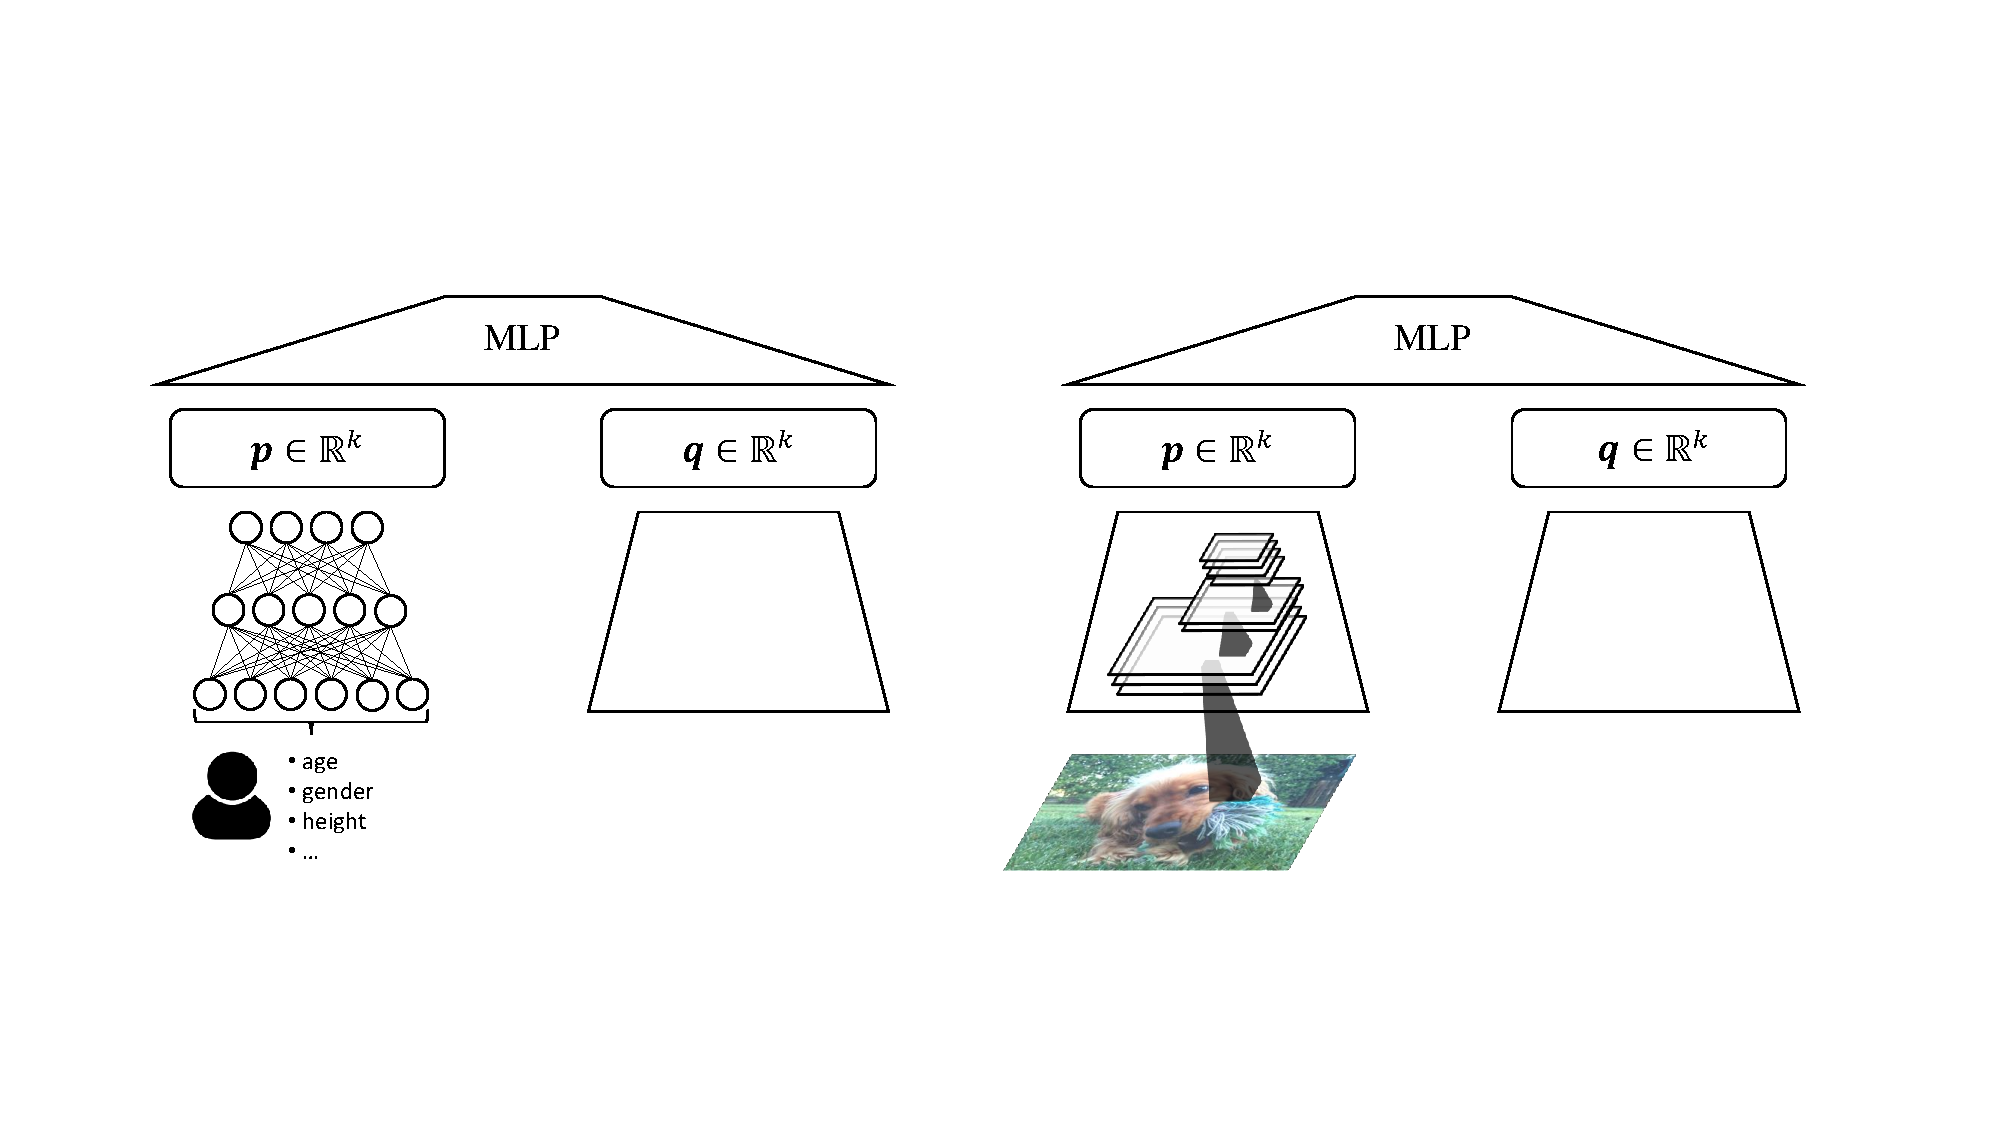
\includegraphics[width=0.9\textwidth,trim = 0 130 0 130,clip]{Dimitris_figures/convnet_plus_fully_connected.pdf}
\end{center}

\end{frame}



\begin{frame}{A flexible neural network architecture 4}
Depending on the type of target variable:

\begin{itemize}
    \item[1.] if the target variable is binary: use BCE
\end{itemize}
\begin{equation}
    \uppercase{{L}}_{{\mathrm{BCE}}} = \sum_{({\mathbf{x}},{\mathbf{t}}, y) \in \mathcal{D}} {y} \log{\hat{y}_{\mathbf{xt}}} + (1 - y)\log{(1 - \hat{y}_{\mathbf{xt}}}).
\end{equation}

\begin{itemize}
    \item[2.] if the target variable is real-valued: use MSE
\end{itemize}
\begin{equation}
    \uppercase{{L}}_{{\mathrm{MSE}}} = \sum_{({\mathbf{x}},{\mathbf{t}}, y) \in \mathcal{D}} {(y - \hat{y}_{\mathbf{xt}})^2}
\end{equation}

\end{frame}


\begin{frame}{A closer look}

\begin{center}
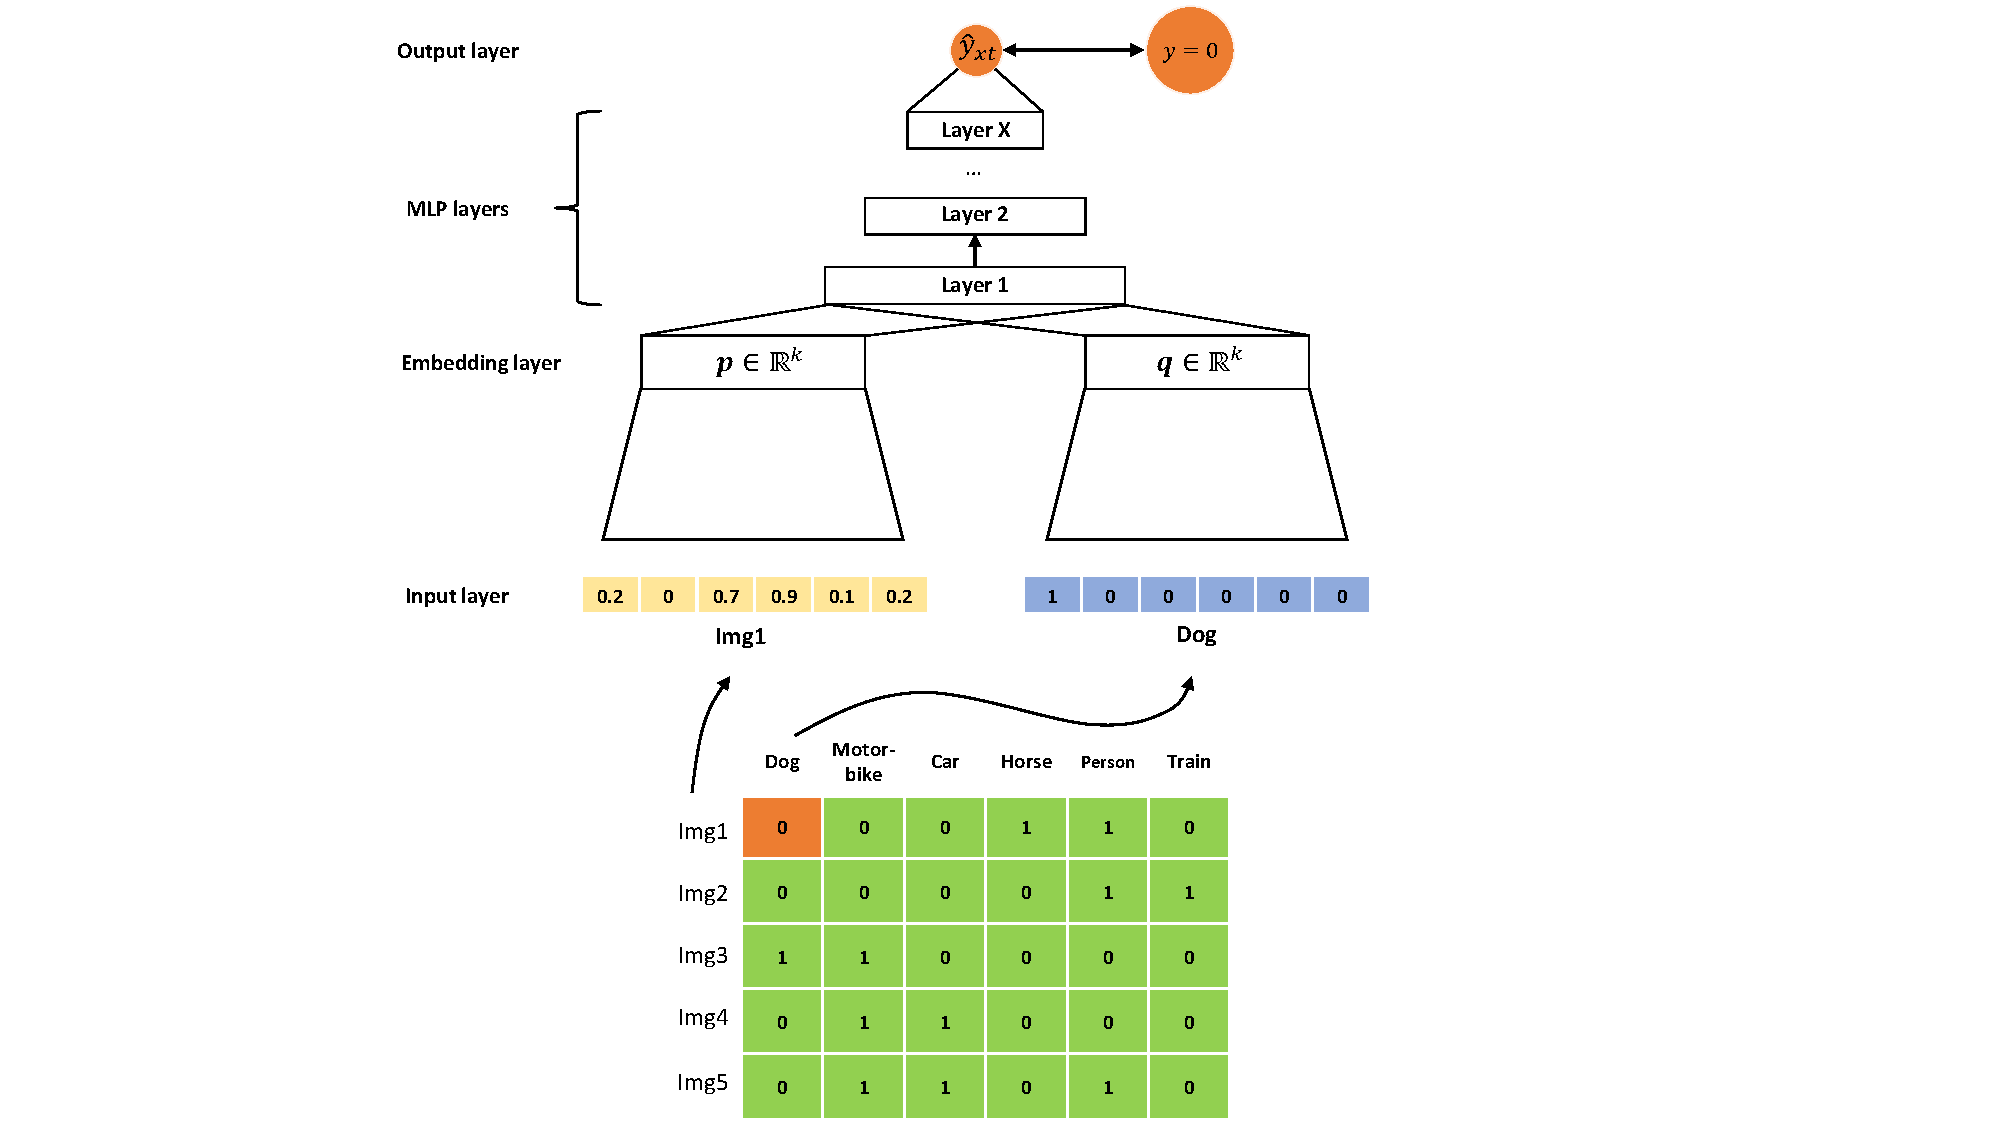
\includegraphics[width=\textwidth,trim = 0 0 0 0,clip]{Dimitris_figures/dual_branch_NN_vertical_v2.pdf}
\end{center}

\end{frame}


\begin{frame}{Validating the framework}
To investigate the effectiveness of the proposed architecture we experimented with multiple datasets from various MTP problem settings.

\begin{columns}

\begin{column}{0.4\textwidth}

\begin{itemize}
\item Multi-label classification
\begin{itemize}
    \item Yeast
    \item Scene
    \item Bibtex
    \item Corel5k
\end{itemize}
\item Multivariate regression

\begin{itemize}
    \item Enb
    \item Jura
    \item Water quality
    \item Oes97
    \item Oes10
    \item Puma8NH
    \item Puma32H
\end{itemize}
\end{itemize}

\end{column}

\begin{column}{0.6\textwidth}


\begin{table}[]
\centering
    \resizebox{\linewidth}{!}{
    \begin{tabular}{c|c|c|c}
    \textbf{Hamming loss} & \textbf{BR(SVM)} & \textbf{MLP} & \textbf{AutoMTP} \\
    \hline
    Yeast         & 0.2392          & 0.2406         & 0.1897\\
    Bibtex       & 0.0158          & 0.0198         & 0.0122\\
    \end{tabular}}
\end{table}

\hskip
\hskip

\begin{table}[]
\centering
    \resizebox{\linewidth}{!}{
    \begin{tabular}{c|c|c|c}
    \textbf{aRRMSE} & \textbf{SVR/target} & \textbf{MLP} & \textbf{AutoMTP} \\
    \hline
    Enb         & 0.1161          & 0.0902         & 0.0.0849\\
    Oes97       & 0.5394          & 0.9905         & 0.9299\\
    Puma32H     & 0.9634          & 0.1009         & 1.0177
    \end{tabular}}
\end{table}

\end{column}

\end{columns}

\end{frame}


\begin{frame}{Validating the framework 2}

\begin{columns}

\begin{column}{0.4\textwidth}

\begin{itemize}
\item Hierarchical multi-label classification
\begin{itemize}
    \item VOC2007
    \item MS COCO
\end{itemize}

\item Matrix completion
\begin{itemize}
    \item Movielens 100k, 1M
\end{itemize}

\item Multi-task learning
\begin{itemize}
    \item Dogs, Birds (crowdsourced annotation)
\end{itemize}

\item Dyadic prediction
\begin{itemize}
    \item DPI-E
    \item DPI-IC
    \item SRN
    \item ERN
\end{itemize}

\end{itemize}
\end{column}

\begin{column}{0.6\textwidth}

\vspace{55mm}

\begin{table}[]
\centering
    \resizebox{0.8\linewidth}{!}{
    \begin{tabular}{c|c|c}
    \textbf{micro-AUC} & \textbf{eBICT} & \textbf{AutoMTP} \\
    \hline
    DPI-E         & 0.8053          & 0.8571\\
    SRN       & 0.8169          & 0.8166\\
    ERN     & 0.8536          & 0.8874
    \end{tabular}}
\end{table}

\end{column}

\end{columns}


\end{frame}


%\begin{frame}
%\frametitle{Many thanks to...}
%\begin{center}
%Michiel Stock, Tapio Pahikkala, Antti Airola, Bernard De Baets,  Krzysztof Dembczynski, Eyke H{\"u}llermeier and Weiwei Cheng for collaborating on this topic!
%
%\vskip18pt
%%\begin{center}
%\begin{minipage}[c]{.8\textwidth}
%\begin{center}
%
%\includegraphics[height=1.5cm]{pics/ms.jpg}
%\hskip0.5cm
%\includegraphics[height=1.5cm]{pics/tp.jpg}
%\hskip0.5cm
%\includegraphics[height=1.5cm]{pics/aa.jpg}
%\hskip0.5cm
%\includegraphics[height=1.5cm]{pics/bdb.jpg}
%\hskip0.5cm \\
%\vspace{1cm}
%\includegraphics[height=1.5cm]{pics/kd.jpg}
%\hskip1cm
%\includegraphics[height=1.5cm]{pics/eh.jpg}
%\hskip1cm
%\includegraphics[height=1.5cm]{pics/wc.jpg}
%\end{center}
%\end{minipage}
%\end{center}
%\end{frame}

%\begin{frame}{Selected references}
%\begin{itemize}
%\item T Pahikkala, M Stock, A Airola, T Aittokallio, B De Baets, W Waegeman A two-step learning approach for solving full and almost full cold start problems in dyadic prediction, ECML/PKDD 2014, 517-532 2014
%\item T. Pahikkala, A. Airola, T. Salakoski, M. Stock, B. De Baets, W. Waegeman, Efficient least-squares algorithms for conditional ranking on relational data, Machine Learning 93, p321-356, 2013
%\item M. Stock, T. Pahikkala, A. Airola, B. De Baets, W. Waegeman, Efficient Pairwise Learning Using Kernel Ridge Regression: an Exact Two-Step Method (Arxiv-preprint)
%\item W. Waegeman, K. Dembczynski, E. H\"ullermeier, A taxonomic review of multi-target prediction methods, in preparation
%\end{itemize}
%\end{frame}
%
%\bibliographystyle{plain}
%\nobibliography{references} 

\end{document}
